\documentclass[draft=false]{oblivoir}
\author{Moon Il-chul \\ \href{mailto:icmoon@kaist.ac.kr}{icmoon@kaist.ac.kr} 
   \and Shin Seung-jae \\ \href{mailto:tmdwo0910@kaist.ac.kr}{tmdwo0910@kaist.ac.kr} }
\setcounter{chapter}{11}
\title{Chapter 11. Variational Inference}
\usepackage{indentfirst}
\usepackage{graphicx}
\graphicspath{ {Figure/} }
\usepackage{hyperref}
\usepackage{amsmath}
\usepackage{amssymb}
\usepackage{amsfonts}
\usepackage{dsfont}
\usepackage[]{algorithm2e}
\usepackage{chngcntr}
\counterwithin{figure}{chapter}
\setcounter{tocdepth}{2}
\setcounter{secnumdepth}{3}
\hypersetup{pdfborder={0 0 0}}
\renewcommand{\thefigure}{\thechapter-\arabic{figure}}
\renewcommand{\theequation}{\thechapter.\arabic{equation}}
\newlength\myindent
\setlength\myindent{5em}

\begin{document}

\maketitle

\tableofcontents

%\chapter{}

\newpage

%-----------------------------------------------------------------
\section{Variational Approximation}
%-----------------------------------------------------------------

\subsection{Variational Transform}
%-----------------------------------------------------------------
Variaitonal Inference를 알아보기에 앞서 Variational Approximation의 방법 중 하나인 Variational Transform에 대해서 알아보겠다. Variational Transform은 어떤 함수 $y=f(x)$를 조금 더 단순한 함수로 표현하는 방법이다.
여기서는 자연로그함수 $y =\ln x$를 예로 들어 설명해보도록 하겠다. 함수 $y = \ln x$를 더 단순한 함수로 표현한 형태인 Variational Transform을 $y = \lambda x + b(\lambda)$라고 하면, 각 $x$값에 대하여 가장 적합한 $\lambda$를 찾는 방법은 다음과 같다.
\begin{equation}
y = min_{x} \left\{ \lambda x + b(\lambda) - \ln x \right\}
\label{eq:11-2-1}
\end{equation}
\begin{equation}
{\frac{d}{dx}}(\lambda x +b(\lambda) -\ln x )=0
\label{eq:11-2-2-1}
\end{equation}
\begin{equation}
\lambda = \frac{1}{x}
\label{eq:11-2-3-1}
\end{equation}
이렇게 특정 $x$에서의 최적화된 Variational Transform 값 $ \lambda = \frac{1}{x}$라는 것을 알았고, 이를 식에 대입하면 $b(\lambda) = -\ln \lambda -1$이라는 것을 알 수 있다. 본 결과에서 미루어 볼 수 있듯이 Variational Transform을 통해 우리는 주어진 변수 $x$에 대해 더욱 간편한 함수를 만들어 내었지만, 본 과정에서 새롭게 등장한 변수 $\lambda$에 대한 처리가 필요해졌음을 알 수 있다.

\begin{figure}[ht] \centering 
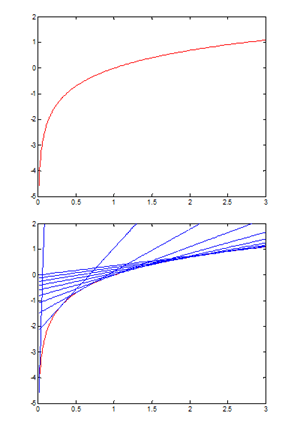
\includegraphics[scale=0.6]{fig11_1.png} 
\caption{ $y = \ln x$의 Variational Transform}
\label{fig:11-1}
\end{figure}

보이는 것처럼 특정 $x$에 대해서는 자연로그함수를 일차함수처럼 표현할 수 있고, 주어진 $x$값에 따라 직선의 기울기와 절편이 달라진다는 것을 확인하였다.

이번에는 Logistic Function $f(x) = \frac{1}{1+e^{-x}}$를 예로 들어 설명해보도록 하겠다. 본 함수는 Sigmoid Function의 종류 중 하나로 Concave (볼록 함수)하지도 Convex (오목 함수)하지도 않은 특징을 가지고 있다. 이는 Variational Transform을 적용하기에 적절하지 않은 함수의 형식인데, 이를 해결하기 위해 이번에는 Logistic Function에 자연로그 함수를 씌운 형태인 $g(x) =ln(f(x))=-\ln (1+e^{-x})$를 Variational Transform 한 후에 다시 지수 함수를 씌워서 원래 함수를 추정하도록 하겠다. 

\begin{equation}
g(x) = min_{\lambda}\left\{{\lambda x -H(\lambda)}\right\}
 \rightarrow 
f(x) = min_{\lambda}\left\{ e^{\lambda x -H(\lambda)}\right\}
\label{eq:11-2-4-1}
\end{equation}

\begin{equation}
H(\lambda) = -\lambda \ln \lambda-(1-\lambda) \ln (1-\lambda)
\label{eq:11-2-5-1}
\end{equation}


\begin{figure}[ht] \centering 
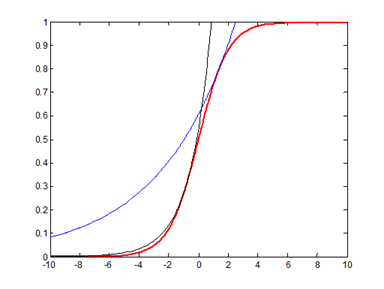
\includegraphics[scale=0.6]{fig11_2.png} 
\caption{ $y = \frac{1}{1+e^{-x}}$의 Variational Transform}
\label{fig:11-2}
\end{figure}
\newpage

\subsection{Convex Duality}
%-----------------------------------------------------------------
이번에는 Variational transform을 Systematic하게 적용한 예시인 Convex Duality에 대해 알아보겠다. 임의의 Concave function $f(x)$를 Linear function으로 표현한다고 하자. 이 과정에서 새로운 함수인 $f^{*}(\lambda)$를 introduce하게 되는데 이 값은 곧 $f(x)$에 대해 근사시킨 linear function의 절편을 의미한다.  
\begin{eqnarray}
f(x) = min_{\lambda}\left\{ \lambda^{T} x - f^{*}(\lambda)\right\}\nonumber\\
 \Leftrightarrow f^{*}( \lambda )=min_{x}\left\{ \lambda^{T}x - f(x)\right\}
\label{eq:11-2-5}
\end{eqnarray}

여기서 주목할 부분은 $f(x)$에 대한 식을 $f^{*}(\lambda)$에 대한 식으로 바꿔 나타내었을 때 $f(x)$와 $f^{*}(\lambda)$의 위치를 바꾸는 것만으로 식을 나타낼 수 있다는 점이다. 이와 같이 함수간에 interchangeable한 특성을 가진 함수를 우리는 Conjugate function 혹은 Dual function이라고 부르는데, 이를 통해 우리는 다음과 같은 추론을 할 수 있다. 

우리는 어떤 복잡한 형태의 함수를 간단한 형태의 함수로 approximation할 수 있다. 다만 이 과정에서 함수의 복잡성은 사라지지 않으며 새롭게 등장한 함수의 Parameter에 이러한 복잡성이 반영되는 것이다.

\subsection{Applying to Probability Function}
%-----------------------------------------------------------------
앞에서 배운 Variational transform과 Convex duality 개념을 토대로 이번엔 확률분포함수 (Probability Function)에 적용시켜 보도록 하겠다. 

결국 확률분포함수 또한 하나의 함수 형태이기 때문에 Variational transform의 적용이 가능하다. 다만 이번에는 확률분포함수의 특성을 감안하여 linear function이 아닌 다른 함수의 형태로 근사시켜보도록 하겠다. 근사의 결과로 나올 함수의 경우 본래 확률분포함수보다 더욱 친숙하고 잘 알려져있는 형태가 될 것이다. 


\begin{figure}[ht] \centering 
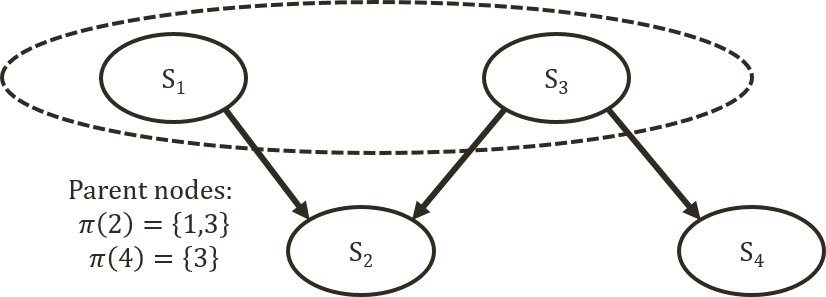
\includegraphics[scale=0.6]{fig11_4.png} 
\caption{ 베이지안 네트워크 예시}
\label{fig:11-4}
\end{figure}

위의 그림은 매우 간단한 베이지안 네트워크의 예시이다. 본 네트워크의 각 node에 대한 Joint probability distribution function을 정의하면 다음과 같다.
\begin{equation}
P(S) = P(S_{1})P(S_{2}|S_{1},S_{3})P(S_{3})P(S_{4}|S_{1}) =\prod_{i}P(S_{i}|S_{\pi(i)})
\label{eq:11-2-6-1}
\end{equation}
\begin{equation}
f(x) = min_{\lambda}\left\{ \lambda^{T}x - f^{*}( \lambda )\right\}\nonumber
\label{eq:11-2-7-1}
\end{equation}

이제 위의 식과 같이 확률분포함수를 Convex duality의 형태로 바꾸어 보자. 바꾼 결과는 다음과 같다. 
\begin{equation}
P(S) = \prod_{i}P(S_{i})|S_{\pi(i)} =min_{\lambda}\prod_{i}P^{U}(S_{i}|S_{\pi(i)}, \lambda^{U}_{i})
\label{eq:11-2-8-1}
\end{equation}

Convex duality를 반영한 식의 경우 기존 P와 다른 $P^U$로 함수가 정의되어 있으며 새로운 Variational parameter $\lambda^{U}_{i}$가 등장함을 알 수 있다. 
\begin{equation}
P(S) = \prod_{i}P(S_{i})|S_{\pi(i)} \leq \prod_{i}P^{U}(S_{i}|S_{\pi(i)},\lambda^{U}_{i})
\label{eq:11-2-9-1}
\end{equation}

\section{Variational Inference}
%-----------------------------------------------------------------
\subsection{Variables of E and H}
%-----------------------------------------------------------------

앞의 장에서는 본래 함수를 조금 더 단순한 형태로 표현하는 방법인 Variational approximation에 대해 알아보았다. 이번 장에서는 배운 개념들을 토대로 Variational inference에 대해 알아보도록 하겠다. 먼저 아래의 그림을 살펴보자.


\begin{figure}[ht] \centering 
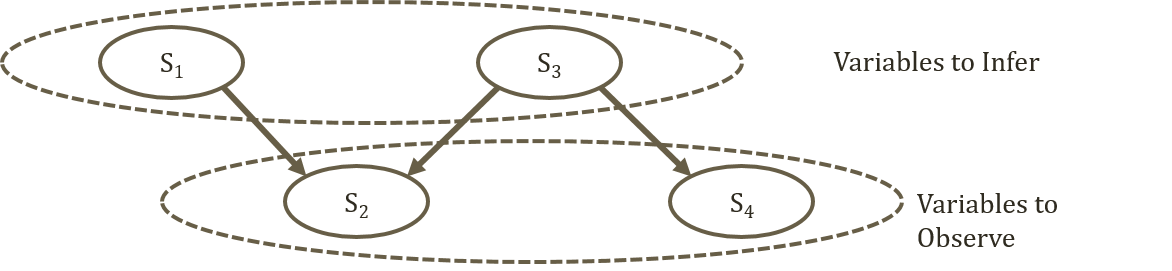
\includegraphics[scale=0.6]{fig11_5.png} 
\caption{베이시안 네트워크 예시}
\label{fig:11-5}
\end{figure}

위의 그림에서 $S_{2}$과 $S_{4}$을 이미 관찰된 Observed variable로,  $S_{1}$과 $S_{3}$을 추론해야할 Latent variable이라고 가정해보자. 만약  Observed variable을 Evidence (E), Latent variable을 Hypothesis(H)라고 칭할 경우 최종 목적은 이미 관찰된 Evidence를 통해 Latent variable, 즉 Hypothesis를 estimate하는 것이 될 것이다.

이미 관찰되었고 고정된 대상인 Evidence와 추론하고 estimate해야할 대상인 Hypothesis 각각은 다음과 같은 성질을 만족한다. 

\begin{equation}
E \cap H =  \phi, E \cup H = S
\label{eq:11-2-10-1}
\end{equation}

이제 Evidence에 대한 확률을 Hidden hypothesis에 대해 marginalize한 다음, Variational approximation을 통해 나타내어 보자. 결과는 다음과 같다. 

\begin{equation}
P(E) = \sum_{H}P(H,E) = \sum_{H}P(S) = \sum_{H}\prod_{i}P(S_{i}|S_{\pi(i)})  \leq  \sum_{H}\prod_{i}P^{U}(S_{i}|S_{\pi(i)},\lambda^{U}_{i})
\label{eq:11-2-11-1}
\end{equation}

\begin{equation}
P(H|E) = P(H,E)/P(E)
\label{eq:11-2-12-1}
\end{equation}

이 과정에서 최종적으로 구하고자 하는 $P(H|E)$는 위와 같이 나타낼 수 있다. 여기서 확률 계산에 어려움을 겪는 부분이 바로 P(E)인데, Hidden variable에 대한 marginalization이 필요해지면서 계산이 매우 복잡해지는 것이다. 우리는 $P(E)$를 Variational inference를 통해 근사함으로써 본 문제를 해결하고자 한다. 

\subsection{Setting the Minimum Criteria}
%-----------------------------------------------------------------
먼저 $P(E)$에 대한 approximation을 위해 $P(E)$의 log-likelihood를 다음과 같이 나타내어 보겠다. 앞의 과정과 마찬가지로 먼저 Hidden variable에 대한 marginalization을 거친 다음 Hidden variable에 대한 Variational distribution $Q$를 도입하였다. 

\begin{equation}
\ln P(E) = \ln \sum_{H}P(H,E)= \ln \sum_{H}Q(H|E)\frac{P(H,E)}{Q(H|E)}
\label{eq:11-2-13}
\end{equation}

이 식은 Jensen's inequality에 의해 다음과 같이 전개된다. log의 경우 전체 영역에 대하여 concave한 특성을 가지고 있기 때문에 전체 함수에 log를 씌운 값이 $\sum$ 내부의 각각의 함수에 log를 씌운 값보다 반드시 크거나 같다. 

\begin{align}
\ln \sum_{H} Q(H|E) \frac{P(H,E)}{Q(H|E)} &  \geq \sum_{H} Q(H|E) \ln \left[ \frac{P(H,E)}{Q(H|E)} \right]\nonumber\\
& = \sum_{H} \left( Q(H|E) \ln P(H,E) - Q(H|E) \ln Q(H|E)\right)\nonumber\\
& = \sum_{H} \left( Q(H|E)\left\{ \ln P(E|H) + \ln P(H)\right\} - Q(H|E)\ln Q(H|E)\right)\nonumber\\
& = \sum_{H} \left( Q(H|E)\ln P(E|H) - Q(H|E) ln\frac{ Q(H|E)}{ P(H)}\right)\nonumber\\
& = E_{Q(H|E)}\ln P(E|H) -KL(Q(H|E)|| P(H))
\label{eq:Q()11-2-5-10}
\end{align}

위의 과정을 거친 결과 $lnP(E)$는 $lnP(E|H)$에 대한 expectation과 $Q(H|E)$, $P(H)$에 대한 KL divergence으로 나타낼 수 있게 된다. 그 결과 위 식은 KL divergence를 최소화할 수록 식의 값이 실제 $lnP(E)$의 값과 가까워짐을 알 수 있다. 

\subsection{Optimizing the Lower Bound}
%-----------------------------------------------------------------
\begin{align}
\ln P(E|\theta) & \geq \sum_{H} \left( Q(H|E,\lambda) \ln P(H,E|\theta) - Q(H|E,\lambda) \ln Q(H|E,\lambda)\right)\nonumber\\
& = \sum_{H} \left( Q(H|E,\lambda)\ln P(E|H,\theta) - Q(H|E,\lambda) ln\frac{ Q(H|E,\lambda)}{ P(H|\theta)}\right)\nonumber\\
& = E_{Q(H|E,\lambda)}\ln P(E|H,\theta) -KL(Q(H|E,\lambda)|| P(H|E,\theta)) 
\end{align}
위 식에서 볼 수 있듯이 Variational distribution을 도입하게 되면서 그에 대한 Variational parameter $\lambda$ 또한 함께 등장하게 된다. 이에 대해 계산되어 나온 식을 우리는 Evidence가 주어졌을 때 이에 대한 Lower Bound, 즉 Evidence Lower bound (ELBO)라고 부르기로 한다. 

\begin{eqnarray}
L(\lambda,\theta) = \sum_{H} \left( Q(H|E,\lambda) \ln P(H,E|\theta) - Q(H|E,\lambda) \ln Q(H|E,\lambda)\right)
\label{eq:Q()11-2-5-1}
\end{eqnarray}

이제 ELBO로 정의된 다음의 식에 대해 최적화하는 방법을 알아보자. ELBO를 구성하는 parameter는 크게 2가지가 있다. 하나는 본래 모델에 존재했던 model parameter $\theta$, 다른 하나는 새롭게 도입한 Variational parameter $\lambda$이다. 이 두 parameter에 대하여 Coordinated ascent method를 통해 ELBO를 최적화할 것이다.  

먼저 ELBO 식의 KL divergence를 최소화하는 방향으로 $\lambda$의 초기값을 세팅해준다. 이는 곧 $Q(H|E,\lambda)$와 $P(H|E,\theta)$를 동일한 값으로 만들어주는 $\lambda$의 값을 찾는 것과 같다. 위의 두 값을 동일한 값으로 취급할 경우 ELBO는 다음과 같이 쓰일 수 있다. 

\begin{align}
&\sum_{H} \left( Q(H|E,\lambda) \ln P(H,E|\theta) - Q(H|E,\lambda) \ln Q(H|E,\lambda)\right)\nonumber\\
 & = \sum_{H} \left( P(H|E,\theta)\ln P(H,E|\theta) -  P(H|E,\theta)\ln  P(H|E,\theta)\right)\nonumber\\
 & = \sum_{H} \left( P(H|E,\theta)\ln P(H|E,\theta)P(E|\theta) -  P(H|E,\theta)\ln  P(H|E,\theta)\right)\nonumber\\
 & = \sum_{H} \left( P(H|E,\theta)\ln P(E|\theta)\right)
 = \ln P(E|\theta)\sum_{H} \left( P(H|E,\theta)\right)
 = \ln P(E|\theta)
\label{eq:Q()11-2-5-2}
\end{align}

결국 ELBO (Evidence Lower Bound)와 $ \ln P(E|\theta)$값이 동일하게 됨으로써 ELBO가 취할 수 있는 최대값을 얻게 되는 것이다. 그 이후에는 Coordinated ascent method에 따라 model parameter인  $\theta$를 update함으로써 이를 최적화하게 된다. 

실제로 ELBO를 적용하는 많은 예시에선 model parameter와 Variational parameter가 각각 여러 개로 주어지는 경우가 많은데, 이 경우 model parameter와 Variational parameter들을 각각 세트로 묶음으로써 model parameter를 변화시킬 땐 Variational parameter를 고정시키고, Variational parameter를 변화시킬 땐 model parameter를 고정시키는 방식으로 parameter 전체를 최적화한다. 이는 앞에서 배운 개념 중 하나인 EM 알고리즘과도 매우 유사한 방식인데 Variational parameter를 학습시키는 단계를 E step, model parameter를 학습시키는 단계를 M step으로 비유할 수 있다. 


%-----------------------------------------------------------------
\subsection{Factorizing Q}
%-----------------------------------------------------------------
이번에는 Variational distribution function Q를 설정하는 방법에 대해 알아보겠다. 앞의 장에서 확인했듯이 $Q(H|E,\lambda)$는 $P(H|E,\theta)$과 그 값이 가까울 수록 최적화에 좋은 조건이며 결국 Q는 $P(H|E,\theta)$와 가까워지는 방향으로 근사를 하게된다. 여기서 주목할 사실은 우리가 임의로 도입한 Q가 특별한 제한조건없이 우리가 원하는 방식으로 정의가 가능하다는 점인데, 이를 이용하여 $Q(H)$를 다음과 같이 나타내고자 한다.

\begin{equation}
Q(H) = \prod_{i\leq|H|}q_{i}(H_{i}|\lambda _{i})
\label{eq:11-2-14}
\end{equation}

다음과 같이 $Q(H)$에 mean field assumption을 적용함으로써 우리는 Hidden variable사이의 연관성 (dependency)를 지울 수 있게 된다. 이를 통해 $Q(H)$를 보다 간단하게 나타낼 수 있음은 물론 훨씬 쉽게 다룰 수 있는 함수의 형태가 되는 것이다. 위의 가정을 적용한 Variational inference를 mean field Variational inference라고 칭하며 본 assumption을 적용한 ELBO를 우리는 다음과 같이 표현할 수 있다.  

\begin{align}
L(\lambda,\theta)\nonumber = {} & \sum_{H} \left( Q(H|E,\lambda) \ln P(H,E|\theta) - Q(H|E,\lambda) \ln Q(H|E,\lambda)\right)\nonumber\\
= {} & \sum_{H}\{\prod_{i\leq|H|}q_{i}(H_{i}|E,\lambda_{i})\ln P(H,E|\theta) - \prod_{i\leq|H|}q_{i}(H_{i}|E,\lambda_{i})\sum_{k\leq|H|}\ln q_{k}(H_{k}|E,\lambda_{k})\}\nonumber\\
= {} & \sum_{H}\prod_{i\leq|H|}q_{i}(H_{i}|E,\lambda_{i})\{\ln P(H,E|\theta) - \sum_{k\leq|H|}\ln q_{k}(H_{k}|E,\lambda_{k})\}\nonumber\\
= {} & \sum_{H_{j}}\sum_{H_{-j}}q_{j}(H_{j}|E,\lambda_{j})\prod_{i\leq|H|,i\neq j}q_{i}(H_{i}|E,\lambda_{i})\{\ln P(H,E|\theta) - \sum_{k\leq|H|}\ln q_{k}(H_{k}|E,\lambda_{k})\} \nonumber\\
= {} & \sum_{H_{j}}\sum_{H_{-j}}q_{j}(H_{j}|E,\lambda_{j})\prod_{i\leq|H|,i\neq j}q_{i}(H_{i}|E,\lambda_{i})\ln P(H,E|\theta)  \nonumber\\
& - \sum_{H_{j}}\sum_{H_{-j}}q_{j}(H_{j}|E,\lambda_{j})\prod_{i\leq|H|,i\neq j}q_{i}(H_{i}|E,\lambda_{i})\left( \sum_{k\neq j,k\leq|H|}\ln q_{k}(H_{k}|E,\lambda_{k})+\ln q_{j}(H_{j}|E,\lambda_{j})\right) \nonumber\\
= {} & \sum_{H_{j}}q_{j}(H_{j}|E,\lambda_{j})\sum_{H_{-j}}\prod_{i\leq|H|,i\neq j}q_{i}(H_{i}|E,\lambda_{i})\ln P(H,E|\theta)-\sum_{H_{j}}q_{j}(H_{j}|E,\lambda_{j})\ln q_{j}(H_{j}|E,\lambda_{j})+C
\label{eq:Q()11-2-5-3}
\end{align}

%-----------------------------------------------------------------
\subsection{Freeform Optimization}
%-----------------------------------------------------------------

\begin{eqnarray}
L(\lambda_{j})\nonumber & = & 
\sum_{H_{j}}q_{j}(H_{j}|E,\lambda_{j})\sum_{H_{-j}}\prod_{i\leq|H|,i\neq j}q_{i}(H_{i}|E,\lambda_{i})\ln P(H,E|\theta)-\sum_{H_{j}}q_{j}(H_{j}|E,\lambda_{j})\ln q_{j}(H_{j}|E,\lambda_{j})+C
\label{eq:Q()11-2-5-4}
\end{eqnarray}
다음과 같이 ELBO를 $\lambda_{j}$에 대한 식으로 나타내어 보았다. 이제 식의 앞항을 새로운 함수인 $\tilde{P}$의 형태로 정의내려 보겠다. 그 결과 j번쨰를 제외한 q에 대한 expectation의 형태로 식이 표현됨을 볼 수 있다. 
\begin{eqnarray}
\ln \tilde{P}(H,E|\theta) & = & 
\sum_{H_{-j}}\prod_{j\leq|H|,j\neq i}q_{j}(H_{j}|E,\lambda_{j})\ln P(H,E|\theta)\nonumber\\ & = & E_{q_{i\neq j}}[\ln P(H,E|\theta)]+C
\label{eq:Q()11-2-5-5}
\end{eqnarray}

이제  $\lambda_{i}$로 ELBO를 정의할 경우 다음과 같이 표현할 수 있다.

\begin{eqnarray}
L(\lambda_{i})\nonumber & = & 
\sum_{H}q_{i}(H_{i}|E,\lambda_{i})\ln \tilde{P}(H,E|\theta)-
\sum_{H}q_{i}(H_{i}|E,\lambda_{i})\ln q_{i}(H_{i}|E,\lambda_{i})+C\nonumber\\ & = & \sum_{H}q_{i}(H_{i}|E,\lambda_{i})\{\ln \tilde{P}(H,E|\theta)/\ln q_{i}(H_{i}|E,\lambda_{i})\}+C
\label{eq:Q()11-2-5-6}
\end{eqnarray}

위의 식에서도 여전히 KL divergence의 형태를 찾을 수 있는데, $\ln \tilde{P}(H,E|\theta)$와 $\ln \tilde{P}(H,E|\theta)$로 이루어진 term이 바로 KL divergence이다. 결국 $\ln \tilde{P}(H,E|\theta)$와 $\ln q_{i}(H_{i}|E,\lambda_{i})$의 값을 같게 만들어줄 때 최적화가 이루어짐을 알 수 있다. 또한 예전의 식과 달리 Q function이 각각의 $q_{i}$로 나타내어져 있기 때문에 각 $q_{i}$에 대해 $E_{q_{i\neq j}}[\ln P(H,E|\theta)]+C$를 maximize하는 방향으로 $\lambda_{i}$를 잡아주는 것이 최적화의 방식이라 할 수 있다. 

%-----------------------------------------------------------------
\section{Examples of Variational inference}
%-----------------------------------------------------------------
%-----------------------------------------------------------------
\subsection{Simple Example Model}
%-----------------------------------------------------------------

지금까지 Variational transformation과 그에 따른 Variational Inference에 대해 알아 보았다. 이제부터는 간단한 확률 모델 예시를 이용하여 본 개념이 어떻게 실제로 적용되는지 살펴 보도록 하겠다. \\

\begin{figure}[ht] \centering 
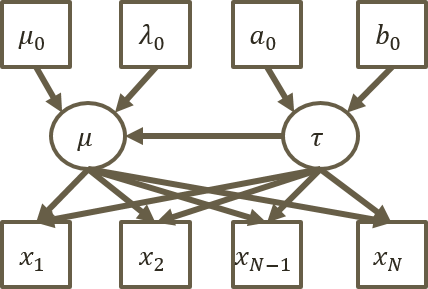
\includegraphics[scale=0.6]{fig11_7.png} 
\caption{확률 예시 모델 }
\label{fig:11-7}
\end{figure}

위의 그림은 아주 간단한 예시의 Graphical model이다. 여기서 관찰 데이터를 $X = (x_{1}, x_{2}, \cdots, x_{N-1}, x_{N})$, variational parameter를 $\mu, \tau $라고 나타내자. 이 경우 $\mu, \tau, x_{i}$의 확률분포와 PDF는 다음과 같다.
\begin{equation}
\mu \sim N(\mu_{0},\frac{1}{\lambda_{0} \tau}), \qquad P(\mu|\tau) = \sqrt{ \frac{\lambda_{0} \tau}{ 2\pi}}e^{- \frac{ \lambda_{0} \tau(\mu-\mu_{0})^{2}}{2}}
\label{eq:11-2-15}
\end{equation}

\begin{equation}
\tau \sim Gamma(a_{0},b_{0}), \qquad P(\tau)= \frac{1}{\Gamma(a_{0})}b_{0}^{a_{0}}\tau^{a_{0}-1}e^{-b_{0}\tau}
\label{eq:11-2-2}
\end{equation}

\begin{equation}
x_{i} \sim N(\mu,\frac{1}{\tau}), \qquad P(x_{i}|\mu, \tau) = \sqrt{\frac{\tau}{2\pi}}e^{- \frac{\tau(x_{i}-\mu)^{2}}{2}}
\label{eq:11-2-3}
\end{equation}

결국 이 과정에서 추론하고자 하는 것은 관측된 각 $x_{i}$에 대한 parameter $\mu$와 $\tau$가 될 것이다. 예시 모델을 살펴보기 전에 Section 1에서 봤던 것처럼 잠재 변수 중 하나인 $H_{i}$와 variational parameter $\lambda$를 $q_{i}$ 분포로 표현하면 다음과 같다.
\begin{equation}
lnq_{i}^{*}(H_{i}|E,\theta_{i}) = ln \overset{\sim}{P}(H,E|\theta)=E_{q_{i \neq j}}[lnP(H,E|\theta)] + C
\label{eq:11-2-4}
\end{equation}

위 과정에서 결국 $ lnP(H,E|\theta)$라는 Hidden과 Evidence에 대한 joint probability distribution에 대한 계산이 필요하다. 이를 위해 위 예시 모델을 다음과 같이 나타내어 보았다. 
\begin{eqnarray}
P(H,E|\theta)\nonumber & = & P(X,\mu,\tau|\mu_{0},\lambda_{0},a_{0},b_{0})\nonumber\\
& = & P(X|\mu,\tau)P(\mu|\tau,\mu_{0},\lambda_{0})P(\tau|a_{0},b_{0})\nonumber\\
& = & 	\prod_{i\leq N}{P(x_{i}|\mu,\tau) P(\mu|\tau,\mu_{0},\lambda_{0})P(\tau|a_{0},b_{0})}
\label{eq:11-2-5-2}
\end{eqnarray}

이제 위의 확률 모델에 대해 Variational distribution과 Variational parameter의 정의가 필요하다. 이 때 새로운 Q function의 Hidden은 $\mu$와 $\tau$가 되며 Evidence는 $x_{i}$가 될 것이다. 이를 나타낸 다음 mean field assumption에 의해 식을 변화시키면 다음과 같은 식이 나오게 된다. 

\begin{equation}
Q(H|E, \lambda) = Q(\mu, \tau | X,\mu^{*},\tau^{*})=q(\mu |X,\mu^{*})q(\tau|X,\tau^{*})
\label{eq:11-2-6}
\end{equation}

그리고 편의를 위해
\begin{equation}
q(\mu |X,\mu^{*}) = q_{\mu}^{*}(\mu), \quad q(\tau|X,\tau^{*}) = q_{\tau}^{*}(\tau)
\label{eq:11-2-7}
\end{equation}
라고 하겠다.

%-----------------------------------------------------------------
\subsection{Calculate an Optimal Variational Parameter}
%-----------------------------------------------------------------
이번 장에서는 mean field assumption에 의해 각각 나누어진 $q_{\mu}^{*}(\mu)$와 $q_{\tau}^{*}(\tau)$에 대해 mean field assumption과 로그의 성질을 이용하여 각각의 확률분포를 알아보겠다. 각 확률변수에 대한 식은 11.24 ~ 11.26을 참조하길 바란다. 아래의 식에서 중요한 점은 $\tau$가 $\mu$에 전혀 영향을 주지 않는 변수라는 점이다. 이를 식에 반영하면 $\tau$에 대한 식은 모두 Constant term으로 처리할 수 있다. 각각 식에 대한 Constant term을 C1 ~ C4로 표현하도록 하겠다.  \\
\begin{align}
lnq_{u}^*(\mu)\nonumber = {} & E_{\tau}\left[ P(X,\mu,\tau|\mu_{0},\lambda_{0},a_{0},b_{0}) \right] +C1\nonumber\\
= {} &	E_{\tau} \left[ln\prod_{i\leq N}{P(x_{i}|\mu, \tau) P(\mu|\tau,\mu_{0},\lambda_{0})P(\tau|a_{0},b_{0})} \right] + C1\nonumber\\
= {} & E_{\tau}\left[ \sum_{i \leq N}\left( \frac{1}{2}(ln \tau -ln2 \pi) - \frac{(x_{i}-\mu)^{2}\tau}{2} \right) \right]\nonumber\\
& + E_{\tau}\left[ \frac{1}{2}(ln \lambda_{0} + ln \tau-ln2 \pi ) - \frac{(\mu -\mu_{0})^{2} \lambda_{0} \tau}{2}\right] + C2\nonumber\\
= {} & E_{\tau}\left[ \sum_{i \leq N} - \frac{(x_{i}-\mu)^{2}\tau}{2} \right] + E_{\tau}\left[ - \frac{(\mu -\mu_{0})^{2} \lambda_{0} \tau}{2}\right] + C3\nonumber\\
= {} & -\frac{E_{\tau}[\tau]}{2}\left[ \sum_{i \leq N} (x_{i}-\mu)^{2} + (\mu -\mu_{0})^{2} \lambda_{0}\right] + C4 \nonumber\\
= {} & -\frac{1}{2}\left[(\lambda_{0} +N)E_{\tau}[\tau] \left(\mu - \frac{\lambda_{0}\mu_{0}+\sum_{i \leq N}x_{i}}{\lambda_{0}+N}   \right)^{2}\right] +C4
\label{eq:11-2-8}
\end{align}

위와 같이 최종적인 식은 $\mu$에 대한 Quadratic function으로 표현할 수 있다. 즉, Variational distribution에 대한 PDF가 위와 같이 정의된 것이다. 그런데 이 형태를 자세히 봐보자. 이는 정규 분포의 PDF에 자연로그를 씌운 꼴과 매우 닮아있다는 것을 알 수 있다. 이에 착안하여 우리는 $ln q_{u}^*(\mu)$가 Normal distribution을 따른다고 가정하자.


$X \sim N(\mu, \sigma^2)$일 때, $X$의 PDF는 
\begin{equation}
p(x) = \frac{1}{\sigma \sqrt{2\pi}}exp\left( -\frac{(x-\mu)^{2}}{2\sigma^{2}} \right)
\label{eq:11-2-9}
\end{equation}
이고, 여기에 자연로그를 씌우면

\begin{equation}
ln(p(x)) = -\frac{1}{2} \left[ \frac{1}{\sigma^{2}}(x-\mu)^{2}\right] +C
\label{eq:11-2-10}
\end{equation}

이다. 따라서 

\begin{equation}
q_{\mu}^{*}(\mu) \sim N \left( \mu| \frac{\lambda_{0}\mu_{0}+\sum_{i \leq N}x_{i}}{\lambda_{0}+N} , \frac{1}{(\lambda_{0}+N)E_{\tau}[\tau]}\right)
\label{eq:11-2-11}
\end{equation}

위 식에서 우리는 $\mu_{0},\lambda_{0}, \sum_{i \leq N}x_{i}, N$은 구할 수 있거나 알고 있는 정보이다.허나, $E_{\tau}[\tau]$는 알고 있지 않다. 이제 $\tau$의 분포를 알기 위해 $lnq_{\tau}^{*}(\tau)$를 계산해보겠다.  $lnq_{\tau}^{*}(\tau)$ 또한 위의 식과 같은 방식으로 구해낼 수 있다. 
\begin{align}
lnq_{\tau}^*(\tau)\nonumber = {} & E_{\tau}\left[ lnP(X,\mu,\tau|\mu_{0},\lambda_{0},a_{0},b_{0}) \right] +C1\nonumber\\
= {} & E_{\mu}\left[ \sum_{i \leq N}\left( \frac{1}{2}(ln\tau -ln2 \pi) - \frac{(x_{i}-\mu)^{2}\tau}{2} \right) \right] + E_{\mu}\left[ \frac{1}{2}(ln \lambda_{0} + ln\tau-ln2 \pi ) - \frac{(\mu -\mu_{0})^{2}\lambda_{0}\tau}{2}\right]\nonumber\\
& + E_{\mu}\left[-ln\gamma(a_{0})+a_{0}lnb_{0}+(a_{0}-1)ln\tau-b_{0}\tau  \right]+C1\nonumber\\
= {} & E_{\mu}\left[ \sum_{i \leq N}\left(-\frac{(x_{i}-\mu)^{2}\tau}{2}\right)\right]+E_{\mu}\left[  - \frac{(\mu -\mu_{0})^{2}\lambda_{0} \tau}{2}\right]+\frac{N}{2}ln\tau+\frac{1}{2}ln\tau+(a_{0}-1)ln\tau-b_{0}\tau+C2\nonumber\\
= {} & -\frac{\tau}{2}E_{\mu}\left[\sum_{i \leq N}(x_{i}-\mu)^2+(\mu-\mu_{0})^2\lambda_{0}\right]+\frac{N}{2}ln\tau+\frac{1}{2}ln\tau+(a_{0}-1)ln\tau-b_{0}\tau+C2\nonumber\\
= {} & -\tau\left(b_{0}+\frac{1}{2}E_{\mu}\left[ \sum_{i \leq N}(x_{i}-\mu)^2+(\mu-\mu_{0})^2\lambda_{0}\right]\right) + (a_{0}+\frac{N+1}{2}-1)ln\tau+C2
\label{eq:11-2-8-2}
\end{align}

$lnq_{\tau}^*(\tau)$은 $\tau$외에 유일한 Hidden variable인 $\mu$에 대한 expectation term으로 표현이 되는데, 이에 대해  $\tau$와 관련없는 수식들을 Constant term으로 분리시킴으로써 식을 위와 같이 전개할 수 있다. 

\begin{equation}
P(X) = \frac{x^{k-1}e^{-\frac{x}{\theta}}}{\theta^k\Gamma(k)}  \;\text{when}\; X \sim Gamma(k,\theta)
\label{eq:11-2-11-2}
\end{equation}

위의 Gamma distribution과 $lnq_{\tau}^*(\tau)$의 식을 비교한 결과 결국 $q_{\tau}^*(\tau)$이 gamma distribution을 따른다고 가정할 수 있다. 이를 통해  $q_{\tau}^*(\tau)$를 다음과 같이 나타낼 수 있다. 
\begin{equation}
q_{\tau}^*(\tau) \sim Gamma\left(\tau|a_{0}+\frac{N+1}{2},b_{0}+\frac{1}{2}E_{\mu}\left[\sum_{i \leq N}(x_{i}-\mu)^2+(\mu-\mu_{0})^2\lambda_{0}\right]\right)\label{eq:11-2-11-3}
\end{equation}

%-----------------------------------------------------------------
\subsection{Coordinated Update}
%-----------------------------------------------------------------
위의 장을 통해 우리는 Variational parameter $q_{\mu}*(\mu)$와 $q_{\tau}*(\tau)$를 각각 다음과 같이 유도해보았다. 

\begin{equation}
q_{\mu}^*(\mu) \sim N \left( \mu| \frac{\lambda_{0}\mu_{0}+\sum_{i \leq N}x_{i}}{\lambda_{0}+N} , \frac{1}{(\lambda_{0}+N)E_{\tau}[\tau]}\right)
= N(\mu|\mu^*,{\lambda^*}^{-1})
\label{eq:11-2-11-4}
\end{equation}
\begin{equation}
q_{\tau}^{*}(\tau)\sim Gamma\left(\tau|a_{0}+\frac{N+1}{2},b_{0}+\frac{1}{2}E_{\mu}\left[\sum_{i \leq N}(x_{i}-\mu)^2+(\mu-\mu_{0})^2\lambda_{0}\right]\right) = Gamma(\tau|a^*,b^*) \label{eq:11-2-11-5}
\end{equation}

위의 식에서 볼 수 있듯이 $q_{\mu}^*(\mu)$의 경우 $E_{\tau}[\tau]$를 추가로 구하고 $q_{\tau}^{*}(\tau)$의 경우 $E_{\mu}[\mu]$와 $E_{\mu}[\mu^2]$를 추가로 구해야 식의 값을 완성시킬 수 있다. 흥미로운 것은 구해야하는 식들의 값을 서로간의 parameter를 이용함으로써 쉽게 구할 수 있다는 점이다. $\tau$에 대한 expectation term은 $q_{\tau}^{*}(\tau)$을 활용하여, $\mu$에 대한 expectation term은 $q_{\mu}^*(\mu)$을 활용하여 어렵지 않게 구할 수 있을 것이다. 이를 이용하여 식에 필요한 expectation term을 다음과 같이 나타내어 보았다. 
\begin{equation}
E_{\tau}[\tau]=\frac{a_{0}+\frac{N+1}{2}}{b_{0}+\frac{1}{2}E_{\mu}\left[\sum_{i \leq N}(x_{i}-\mu)^2+(\mu-\mu_{0})^2\lambda_{0}\right]}=\frac{a^*}{b^*}:\;\text{Need} \; E_{\mu}[\mu] \; \text{and} \; E_{\mu}[\mu^2]
\label{eq:11-2-11-6}
\end{equation}
\begin{equation}
E_{\mu}[\mu]=\frac{\lambda_{0}\mu_{0}+\sum_{i \leq N}x_{i}}{\lambda_{0}+N}=\mu^*:\;\text{Don't need anything}
\label{eq:11-2-11-7}
\end{equation}
\begin{equation}
E_{\mu}[\mu^2]=\frac{1}{(\lambda_{0}+N)E_{\tau}[\tau]}+(\frac{\lambda_{0}\mu_{0}+\sum_{i \leq N}x_{i}}{\lambda_{0}+N})^2=\lambda^{*-1}+(\mu^*)^2: \;\text{Needs} E_{\tau}[\tau]
\label{eq:11-2-11-8}
\end{equation}

위와 같이 Variational distribution와 parameter의 형태는 물론 식의 완성을 위해 필요한 expectation term에 대한 식도 구해보았다. 이제 우리는 완성된 식을 바탕으로 서로간에 interlocking된 parameter $q_{\mu}^*(\mu)$와 $q_{\tau}^{*}(\tau)$를 번갈아가며 학습시키는 Coordinated ascent optimization 방식으로 최적화를 진행할 것이다. 
%-----------------------------------------------------------------
\subsection{Algorithm for the Parameter Update}
%-----------------------------------------------------------------
\begin{figure}[ht] \centering 
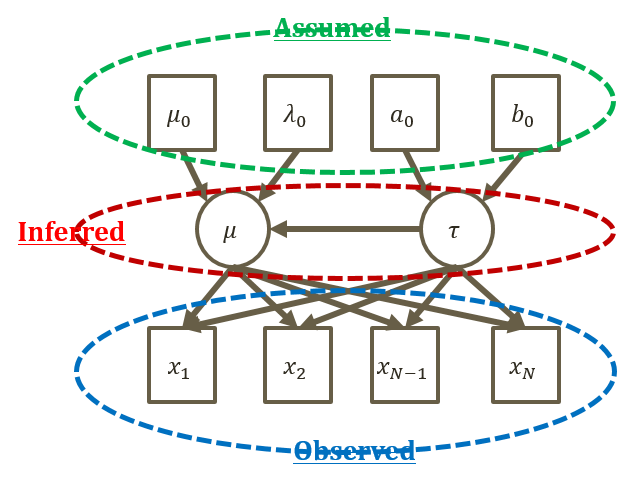
\includegraphics[scale=0.6]{fig11_8.png} 
\caption{Graphic model of baysian network example}
\label{fig:11-8}
\end{figure}
위 Graphic model에 대하여 우리가 infer해야 할 Hidden인 $\mu$와 $\tau$에 대해 inference해가는 과정은 다음과 같다. 
\begin{equation}
a^{*}=a_{0}+\frac{N+1}{2}\;,\; \mu^*=\frac{\lambda_{0}\mu_{0}+\sum_{i \leq N}x_{i}}{\lambda_{0}+N}
\label{eq:11-2-11-9}
\end{equation}
$\lambda^*$의 경우 $b^{*}$와 interlocking되어있기 때문에 값을 바로 구할 수 없다. 일단 arbitrary number로 $\lambda^*$의 값을 결정한 다음 이를 $b^{*}$의 식에 대입하고 $b^{*}$의 값을 또 다시 $\lambda^*$의 식에 대입하며 두 값이 특정 값으로 Converge할 때까지 이를 반복해준다. 각 값에 대한 식은 다음과 같다. 
\begin{equation}
b^{*}=b_{0}+\frac{1}{2}E_{\mu}\left[\sum_{i \leq N}(x_{i}-\mu)^2+(\mu-\mu_{0})^2\lambda_{0}\right]
\label{eq:11-2-11-10}
\end{equation}
\begin{equation}
\lambda^{*}=(\lambda_{0}+N)E_{\tau}[\tau]
\label{eq:11-2-11-11}
\end{equation}
두 값이 특정한 값으로 Converge했을 때 비로소 우리는 approximate된 $\mu$와 $\tau$의 값을 구할 수 있다.
%-----------------------------------------------------------------
\subsection{Generalized Step-By-Step Instruction}
%-----------------------------------------------------------------
아래의 figure는 Probabilistic Model에 대한 Variational inference 과정을 순서대로 나타낸 것이다. 

\begin{figure}[ht] \centering 
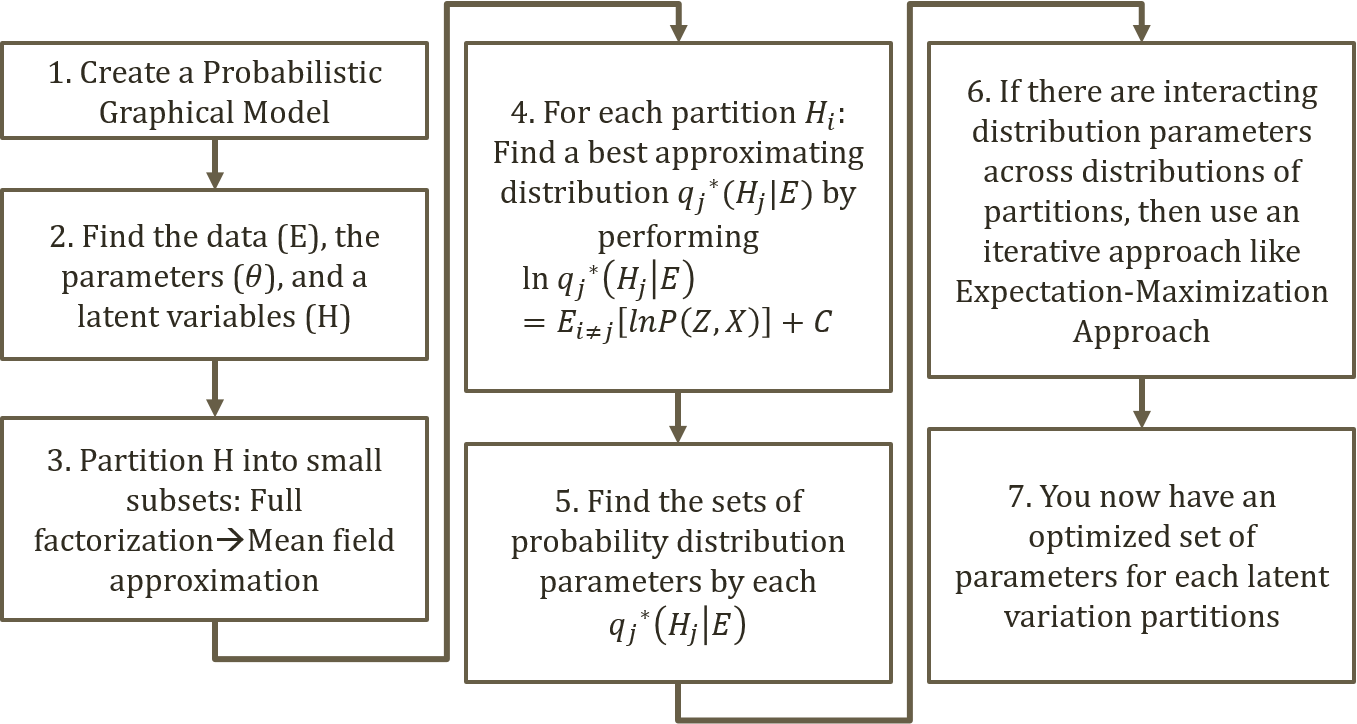
\includegraphics[scale=0.4]{fig11_9.png} 
\caption{Generalized Step-By-Step Instruction}
\label{fig:11-9}
\end{figure}

%-----------------------------------------------------------------
\section{Variational inference of Latent Dirichlet Allocation}
%-----------------------------------------------------------------
이번 장에서는 Topic model의 종류 중 하나인 LDA (Latent Dirichlet Allocation)에 Variational inference를 적용시켜보도록 하겠다. 

%-----------------------------------------------------------------
\subsection{Detour: Latent Dirichlet Allocation}
%-----------------------------------------------------------------
본격적으로 VI를 적용해보기 앞서, 이미 배운 바 있는 LDA에 대해 다시 한번 정리해보도록 하겠다. 

LDA (Latent Dirichlet Allocation)는 text data에 대해 probability distribution을 기준으로 하여 군집을 형성하는 soft clustering 방식의 모델이다. 
아래의 그림에서 볼 수 있듯이 LDA는 텍스트를 모아놓은 집단인 corpus의 structure까지 반영할 수 있는 장점이 있으며, 미리 알고 있는 주제별 단어수 분포를 바탕으로 주어진 문서에서 발견된 단어 수 분포를 분석하는 방식으로 text corpus에 대한 주제를 예측한다.

\begin{figure}[ht] \centering 
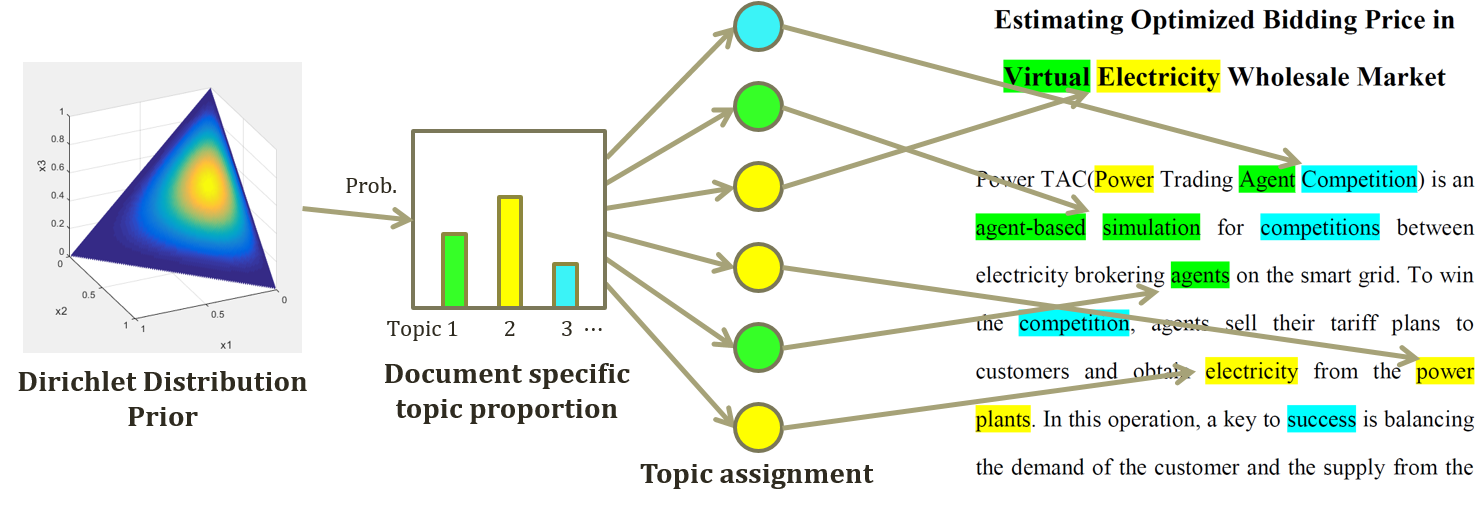
\includegraphics[scale=0.5]{fig11_10.png} 
\caption{Graphic description of LDA}
\label{fig:11-10}
\end{figure}

아래의 그림은 LDA의 Graphic model이다. M은 Document의 총 개수를 나타낸다. 또, N은 Document i 속에 있는 단어의 개수를 나타낸다. $(1 \leq i \leq M)$ 마지막으로 K는 우리가 추출하고자 하는 topic의 갯수를 나타낸다. 

\begin{figure}[ht] \centering 
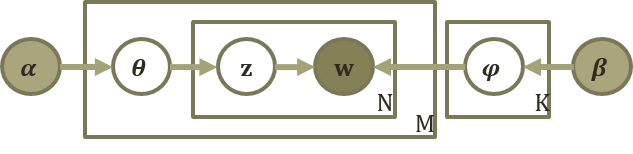
\includegraphics[scale=0.8]{fig11_11.png} 
\caption{Graphic model of LDA}
\label{fig:11-11}
\end{figure}

또한 모델 내의 변수들이 가지는 분포와 의미는 다음과 같다. 

\begin{eqnarray*}
&\theta_{i} \sim Dir(\alpha), i \in \{1,...,M\}\nonumber\\
&\varphi_{k} \sim Dir(\beta), k \in \{1,...,K\}\nonumber\\
&z_{i,l} \sim Mult(\theta_{i}), i \in \{1,...,M\}, l in \{1,...,N\}\nonumber\\
&w_{i,l} \sim Mult(\varphi_{z_{i,l}}), i \in \{1,...,M\},l \in \{1,...,N\}\nonumber
\end{eqnarray*}

단어 w는 $ \varphi $에 의한 Multinomial distribution (word-topic distribution)의 분포를 따르며 토픽 z는 $\theta$에 의한 Multinomial distribution (document-topic distribution)의 분포를 따른다. 또한 $ \varphi $는 hyper-parameter $\beta$에 의한 dirichlet distribution의 영향을 받으며 $\theta$는  hyper-parameter $\alpha$에 의한 dirichlet distribution의 영향을 받는 구조라 할 수 있다. 

%-----------------------------------------------------------------
\subsection{Evidence Lower Bound of LDA}
%-----------------------------------------------------------------
LDA에 Variational inference를 적용하려면 먼저 최적화의 대상이 되는 LDA의 ELBO(Evidence Lower Bound)를 구해야 한다. 아래는 일반적인 상황에서의 ELBO에 대한 식을 나타낸 것이다. 

\begin{eqnarray}
\ln P(E|\theta) & \geq & \sum_{H} \left( Q(H|E,\lambda) \ln P(H,E|\theta) - Q(H|E,\lambda) \ln Q(H|E,\lambda)\right)\nonumber\\
& = & \sum_{H} \left( Q(H|E,\lambda)\ln P(E|H,\theta) - Q(H|E) ln\frac{ Q(H|E,\lambda)}{ P(H|\theta)}\right)\nonumber
\end{eqnarray}

위의 식에서 E는 Evidence로 이미 관측된 관측치이며 $\theta$의 경우 추론을 필요로 하는 parameter이다. 고로 LDA 모델에서는 관측치 E가 w, $\theta$가 parameter $\alpha$, $\beta$를 의미하게 된다. 위의 과정을 그대로 가지고 와서 이번엔 LDA의 ELBO를 구해보도록 하겠다. jenson's inequality 와 bayesian network factorization을 통해 어렵지 않게 식을 전개시켜나갈 수 있다. 

\begin{align}
\ln P(w|\alpha,\beta) \geq {} & \int\sum_{z}q(\theta,z|\tau,\phi)log\frac{P(\theta,z,w|\alpha,\beta)}{q(\theta,z|\tau,\phi)}d\theta\nonumber\\
= {} & \int\sum_{z}q(\theta,z|\tau,\phi)log P(\theta,z,w|\alpha,\beta)d\theta - \int\sum_{z}q(\theta,z|\tau,\phi)log q(\theta,z|\tau,\phi)d\theta \nonumber\\
= {} & \int\sum_{z}q(\theta,z|\tau,\phi)log P(\theta|\alpha)d\theta + \int\sum_{z}q(\theta,z|\tau,\phi)log q(z|\theta)d\theta \nonumber\\
& + \int\sum_{z}q(\theta,z|\tau,\phi)log P(w|z,\beta)d\theta - \int\sum_{z}q(\theta,z|\tau,\phi)log q(\theta,z|\tau,\phi)d\theta \nonumber\\
= {} & E_{q}(logP(\theta|\alpha))+E_{q}(log P(z|\theta))+E_{q}(logP(w|z,\beta))+H(q) \;(H(p) \overset{\text{def}}{=} -\sum_{i}p(x_{i})logp(x_{i}))\nonumber\\
\overset{\text{def}}{=} {} & L(\gamma,\phi|\alpha,\beta)
\label{eq:Q()11-2-5-7}
\end{align}

위의 식에서 눈여겨볼 부분은 q를 하나의 확률분포로 가정함으로써 각각의 식을 expectation term으로 표현할 수 있다는 점이다. 단, $H(q)$의 경우 expectation term이 아닌 다른 형태로 표기하였는데, 위의 식이 entropy의 식과 동일하기 때문에 위와 같이 표기하였다. 

또한 임의로 식에 반영해준 variational distribution q에 대해 mean field assumption 을 적용하여 $q(\theta,z|\gamma,\phi)$대신  $q(\theta|\gamma)q(z|\phi)$으로 표현해줌으로써 최종 ELBO식을 Variational parameter와 model parameter에 기반한 식 $L(\gamma,\phi|\alpha,\beta)$으로 만들어줄 수 있게 된다. Mean field assumption을 적용한 $q$ distribution에 대한 graphic model을 다음과 같이 나타낼 수 있다.

\begin{figure}[ht] \centering 
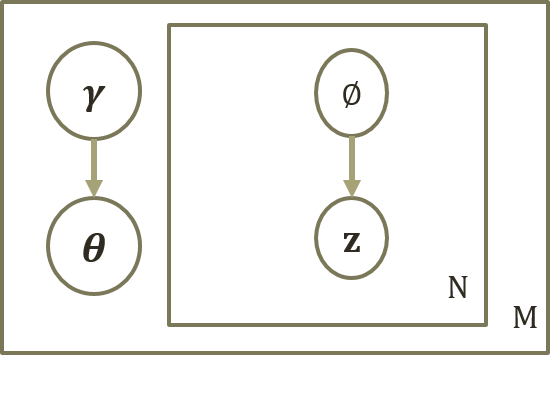
\includegraphics[scale=0.7]{fig11_12.png} 
\caption{Graphic model of variational distribution q}
\label{fig:11-12}
\end{figure}

graphic model에서 볼 수 있듯이 우리는 mean field assumption을 통해 
각각의 변수에 대한 연관성을 끊었음을 알 수 있다. 이를 통해 우리는 조금 더 간편하게 변수간의 관계를 정의할 수 있게 된다. 

%-----------------------------------------------------------------
\subsection{Detour : Dirichlet distribution}
%-----------------------------------------------------------------
앞의 단원에서 배운 바 있는 Dirichlet distribution에 대하여 다시 한번 개략적인 소개를 하고 넘어가도록 하겠다. 

Beta distribution이 Binomial distribution에 대한 conjugate prior로 쓰인다면 Dirichlet distribution은 Multinomial distribution에 대한 conjugate prior로 쓰이는 것으로 잘 알려져 있다. 간단히 말해 dirichlet distribution을 Beta distribution에 대한 확장 버전으로 이해해도 무방하다.

* Dirichlet distribution
\begin{gather*}
P(x_{1},...,x_{K}|\alpha_{1},...,\alpha_{K}) = \frac{\Gamma(\sum^{K}_{i=1}\alpha_{i})}{\Pi^{N}_{i=1}\Gamma(\alpha_{i})}{x_{i}}^{\alpha_{i}-1}\\
x_{1},...,x_{K-1} > 0 \\
x_{1}+...+x_{K-1} < 1 \\
x_{K}=1-x_{1}-x_{2}-...-x_{K-1}\\
\alpha_{i} > 0 \; (\text{for} \; 1 \leq i \leq K)
\end{gather*}

위에서 볼 수 있듯이 distribution을 이루는 변수 $x_{1},...,x_{K-1},x_{K}$가 probability axiom를 잘 만족함을 알 수 있다. 위의 특징을 이용하여 multinomial distribution에 대한 prior distribution으로 dirichlet distribution을 이용할 수 있는 것이다.
%-----------------------------------------------------------------
\subsection{Detour : Exponential Family}
%-----------------------------------------------------------------
Exponential Family(지수분포 족) 라고 일컬어지는 개념과 특성을 이용함으로써 우리는 mathematical derivation을 좀 더 편리하게 수행할 수 있다. 이번에는 LDA의 VI(Variational inference) 적용 과정에서 쓰일 Exponential Family에 대해 알아보도록 하겠다. 

우리는 변수 $x$와 파라미터 $\theta$에 대한 식이 다음과 같은 형태로 표현될 수 있을 때 이를 Exponential Family(지수분포 족)의 특성을 가진다고 이야기한다. 

\begin{gather*}
P(x\mid \theta)=h(x)exp(\eta(\theta)\cdot T(x)-A(\theta))\\
\text{Sufficient statistics} : T(x) \qquad
\text{Natural parameter} : \eta(\theta)\\
\text{Underlying measure} : h(x) \qquad
\text{Log normalizer} : A(\theta)\\
\end{gather*}

underlying measure로 선언된 h(x)와 Log normalizer $A(\theta)$의 경우 확률의 합을 1로 만들기 위한 normalizing value이며 중요한 의미를 갖는 부분은 Sufficient statistics $T(x)$이다. Sufficient statistics는 말 그대로 statistical data x의 전체를 설명해낼 수 있는 함수이자 statistics라는 뜻이다. 즉, $T$라는 함수를 통해 받아들인 $x$의 정보를 활용하겠다는 의미를 담고 있다. $\eta(\theta)$의 경우 natural parameter로 불리는데 $\theta$라는 parameter가 주어진 수식에 수학적으로 잘 적용될 수 있도록 역할을 하는 식이라 볼 수 있다. 

다음으로 우리에게 친숙한 몇가지 확률분포를 대상으로 Exponential Family 식으로 변환이 가능한 지를 보도록 하겠다. \\

1. Normal Distribution
\begin{gather*}
P(x\mid \mu,\sigma) = \frac{1}{\sqrt{2\pi\sigma^2}}exp(-\frac{(x-\mu)^2}{2\sigma^2})=\frac{1}{\sqrt{2\pi\sigma^2}}exp(-\frac{(x^2-2\mu x+\mu^2)}{2\sigma^2})\nonumber\\
\text{Sufficient statistics} : {(x,x^2)}^T \quad
\text{Natural parameter} : {(\frac{\mu}{\sigma^2},-\frac{1}{2\sigma^2})}^T\\
\text{Underlying measure} : \frac{1}{\sqrt{2\pi}} \quad
\text{Log normalizer} : \frac{\mu^2}{2\sigma^2}+log|\sigma|
\end{gather*}

위의 식에서 볼 수 있듯이 Normal Distribution의 경우 Exponential family의 형태를 만족함을 알 수 있다. 또한 Log normalizer의 $log|\sigma|$의 경우 exponential의 앞에 위치한 $\sigma$가 exponential 안에 들어가면서 log가 씌워졌음을 알 수 있다. \\

2. Dirichlet Distribution
\begin{eqnarray*}
&P(x_{1},...,x_{K}|\alpha_{1},...,\alpha_{K}) = \frac{\Gamma(\sum^{K}_{i=1}\alpha_{i})}{\Pi^{N}_{i=1}\Gamma(\alpha_{i})}{x_{i}}^{\alpha_{i}-1}\nonumber  \\
&\text{Sufficient statistics} : {(logx_{1},...,logx_{K})}^T\nonumber\\
&\text{Natural parameter} : {(a_{1}-1,...,a_{K}-1)}^T\nonumber\\
&\text{Underlying measure} : 1\nonumber\\
&\text{Log normalizer} : -log\Gamma(\sum^{K}_{i=1}\alpha_{i})+log\Pi^{N}_{i=1}\Gamma(\alpha_{i})\nonumber
\label{eq:11-2-11-12}
\end{eqnarray*}

위와 같이 Dirichlet Distribution 또한 Exponential family의 형태를 만족한다. 다만 식 내에 exponential이 정의되어 있지 않기 때문에 식에 log를 씌우고 이에 대해 exponential을 다시 씌우는 방식을 통해 exponential family의 형태를 갖춰주어야 한다. \\

* Derivative of log normalizer $\rightarrow$ Moments of sufficient statistics\\

\begin{eqnarray}
\frac{d}{d\eta}A(\eta) & = & 
\frac{d}{d\eta}log\int h(x)exp\{\eta^{T}T(x)\}dx = \frac{\int T(x)h(x)exp\{\eta^{T}T(x)\}dx}{\int h(x)exp\{\eta^{T}T(x)\}dx}\nonumber\\
& = & \frac{\int T(x)h(x)exp\{\eta^{T}T(x)\}dx}{exp(A(\eta))}=\int T(x)h(x)exp\{\eta^{T}T(x)-A(\eta)\}dx = E_{p}|T(x)|\nonumber\\
\label{eq:Q()11-2-5-8}
\end{eqnarray}

위의 식은 log normalizer 로 정의된 $a(\eta)$를 $\eta$에 대해 미분할 경우 sufficient statistics $T(x)$의 moments의 형태가 됨을 보여주는 식이다. 미분한 결과에서 볼 수 있듯이 마지막 식이 $T(x)$와 식 내 확률분포인 PDF의 곱에 대한 적분식으로 주어짐을 알 수 있다. 이는 $T(x)$에 대한 확률분포 p의 expectation term의 형태가 되며 곧 $T(x)$의 moments와 형태가 같아짐을 알 수 있다. 우리는 LDA의 VI 적용과정에서 이를 이용할 것이다. 

%-----------------------------------------------------------------
\subsection{Derivation of \texorpdfstring{$E_{q}(log P(\theta|\alpha))$}{Lg}}
%-----------------------------------------------------------------
\begin{equation}
L(\gamma,\phi|\alpha,\beta)\nonumber = E_{q}(log P(\theta|\alpha))+E_{    q}(log P(z|\theta))+E_{q}(log P(w|z,\beta))+H(q)\nonumber
\end{equation}
이제 우리는 LDA의 식을 바탕으로 variational parameter인 $\gamma$,$\phi$와 model parameter인 $\alpha$와 $\beta$를 학습시킬 것이다. 허나, 현재 제시된 ELBO의 식 형태는 위와 같이 expectation term, entropy 형식으로서 바로 계산을 할 수 있는 형태가 아니기에 이를 각각의 parameter에 대해 바로 계산할 수 있는 형태로 나타내보고자 한다. 첫번쨰로 LDA의 ELBO 식 중 첫번째 항인 $E_{q}(log P(\theta|\alpha))$의 형태를 바꾸어 보겠다. 
\begin{eqnarray*}
&P(x_{1},...,x_{K}|\alpha_{1},...,\alpha_{K}) = \frac{\Gamma(\sum^{K}_{i=1}\alpha_{i}}{\Pi^{N}_{i=1}\Gamma(\alpha_{i})}{x_{i}}^{\alpha_{i}-1}\nonumber\\
\label{eq:Q()11-2-5-9}
\end{eqnarray*}
위의 식은 dirichlet distribution에 대한 pdf이다. LDA상의 $\theta$ 또한 Dir($\alpha$)를 따르기 때문에 이를 활용하여 식을 전개시킬 수 있다. 
\begin{eqnarray}
E_{q}(log P(\theta|\alpha))& = & E_{q}\left(\sum^{M}_{d=1}\sum^{K}_{i=1}(a_{i}-1)log\theta_{d,i}+ log\Gamma\left(\sum^{K}_{i}\alpha_{i}\right)-\sum^{K}_{i}log\Gamma(\alpha_{i})\right)\nonumber\\
& = & \sum^{M}_{d=1}\sum^{K}_{i=1}(a_{i}-1)E_{q}(log\theta_{d,i})+log\Gamma\left(\sum^{K}_{i}\alpha_{i}\right)-\sum^{K}_{i}log\Gamma(\alpha_{i})\nonumber\\
\end{eqnarray}

식의 형태를 바꾼 후에도 문제가 되는 부분이 있다. 바로 expectation term $E_{q}(log\theta_{d,i})$인데, 앞에서 논했듯이 expectation term의 경우 바로 계산할 수 있는 형태의 식이나 함수로 바꿔주어야 한다. 

식을 전개하는 과정에서 참고해야할 부분이 있다. 바로 $q(\theta,z|\gamma,\phi)$의 식을 변화시키는 부분인데, 아래 식을 보자. 원래 식에 대해  mean field assumption을 적용하고 식과 연관성이 있는 부분만을 marginalize하여 Variational distribution을 매우 간단하게 나타냈음을 알 수 있다.\\
\begin{equation}
E_{q(\theta,z|\gamma,\phi)}(log\theta_{d,i})=E_{q(\theta|\gamma)q(z|\phi)}(log\theta_{d,i})=E_{q(\theta|\gamma)}(log\theta_{d,i})
\end{equation}
또한 variational distribution $q$가 우리가 임의로 정의한 distribution이라는 점을 이용하여 $q(\theta|\gamma)$ 또한 $P(\theta|\alpha)$가 따르는 dirichlet distribution을 따른다고 가정하자. 이를 이용하여 Sufficient statistics와 Log normalizer를 다음과 같이 나타낼 수 있다.
\begin{eqnarray*}
&\text{Sufficient statistics} = (log\theta_{d,1},...,log\theta_{d,K})^{T}\nonumber\\
&\text{Log normalizer} = -log\Gamma(\sum^{K}_{i=1}\gamma_{d,i})+log\Pi^{K}_{i=1}\Gamma(\gamma_{d,i})\nonumber
\end{eqnarray*}
그 다음, Derivative of log normalizer가 Sufficient statistics의 Moments를 의미한다는 것을 이용하여 다음의 식을 쓸 수 있다. 

\begin{eqnarray}
E_{q(\theta|\gamma)}(log\theta_{d,i})\nonumber & = &\frac{d}{d\gamma_{d,i}}\left(-log\Gamma\left(\sum^{K}_{i=1}\gamma_{d,i}\right)+log\Pi^{K}_{i=1}\Gamma(\gamma_{d,i})\right)\nonumber\\ 
& = & -\psi\left(\sum^{K}_{i=1}\gamma_{d,i}\right)+\psi(\gamma_{d,i})
\end{eqnarray}


결국 $E_{q(\theta|\gamma)}(log\theta_{d,i})$은 digamma function의 형태로 정의할 수 있게 되고 이를 원래 식 대신 집어넣음으로써 바로 계산할 수 있는 형태의 식을 만들 수 있게 된다.\\

* digamma function
\begin{equation}
\psi(\gamma_{d,i}) = \frac{d}{d\gamma_{d,i}}log\Gamma(\gamma_{d,i}) = \frac{\Gamma^{'}(\gamma_{d,i})}{\Gamma(\gamma_{d,i})}\nonumber
\end{equation}

위는 digamma distribution에 대한 식이다. digamma function은 컴퓨터 언어 내 mathematical library를 이용하여 함숫값을 계산할 수 있다. 따라서 digmma fucntion으로 표현된 식은 계산할 수 있는 형태의 식이다.

\begin{equation}
E_{q}(logP(\theta|\alpha)) = \sum^{M}_{d=1}\sum^{K}_{i=1}(\alpha_{i}-1)\left(-\psi\left(\sum^{K}_{i=1}\gamma_{d,i}\right)+\psi(\gamma_{d,i})\right)+log\Gamma\left(\sum^{K}_{i=1}\alpha_{i}\right)-\sum^{K}_{i=1}log\Gamma(\alpha_{i})
\end{equation}

앞에서 배운 내용을 실제로 적용하여 $E_{q}(log P(\theta|\alpha))$을 다음과 같이 바로 계산이 가능한 식으로 바꿔 보았다.  
%-----------------------------------------------------------------
\subsection{Derivation of \texorpdfstring{$E_{q}(log P(z|\theta))$}{Lg}  and \texorpdfstring{$E_{q}(log P(w|z,\beta))$}{Lg}}
%-----------------------------------------------------------------
이번에는 ELBO의 두번째, 세번째 항인 $E_{q}(log P(z|\theta))$ 와 $E_{q}(log P(w|z,\beta))$에 대한 derivation을 구해보도록 하겠다. \\

$P(z|\theta)$에서 $\theta$의 경우 각 문서에 대한 확률 분포를 나타내기 때문에 $\theta_{d}$에서 $d$는 1부터 $M$까지의 값을 가진다. 또한 z의 경우 각 문서에 포함된 단어들에 대한 확률 분포를 나타내며 $z_{d,n}$에서 $n$은 1부터 문서 $d$의 단어 개수를 나타내는 $N_{d}$까지의 값을 가진다. 또한 각각의 문서 $\theta$ 와 단어 $z$에 assign될 수 있는 topic은 1부터 $K$까지의 값을 가질 것이다. $z_{d,n}$이 독립동일분포(identical and independent distribution, i.i.d)임을 이용하여 다음과 같이 나타낼 수 있다.

\begin{eqnarray}
E_{q}(log P(z|\theta))\nonumber & = &  \sum^{M}_{d=1}\sum^{N_{d}}_{n=1}E_{q}(logP(z_{d,n}|\theta_{d}))\nonumber = \sum^{M}_{d=1}\sum^{N_{d}}_{n=1}\sum^{K}_{i=1}E_{q}(logP(z_{d,n,i}|\theta_{d,i}))\nonumber
\end{eqnarray}

우리가 binomial distribution에서 특정 사건이 일어날 확률을 distribution의 parameter인 $\theta$라고 나타내었던 것처럼 multinomial distribution을 가지는 $P(z_{d,n,i}=1|\theta_{d,i})$의 확률을 우리는 $\theta_{d,i}$라고 나타낼 수 있다. 허나, 본 확률은 $z_{d,n,i}$의 값이 1을 가지는, 말 그대로 $z_{d,n}$이 i번째 topic에 assign된 경우에만 효력을 가지므로 $z_{d,n,i}$이 1일 때만 값을 가질 수 있게 ${\theta_{d,i}}^{z_{d,n,i}}$으로 표현할 수 있도록 한다.  그 다음 Section 4.5와 같은 방식으로 $q(z|\phi)$ 또한 $P(z|\theta)$가 따르는 multinomial distribution을 따른다고 가정하고 mean field assumption을 적용하여 식을 전개하면 다음과 같은 결과가 나오게 된다.

\begin{eqnarray}
E_{q}(log P(z|\theta)) & = &  \sum^{M}_{d=1}\sum^{N_{d}}_{n=1}E_{q}(logP(z_{d,n}|\theta_{d})) = \sum^{M}_{d=1}\sum^{N_{d}}_{n=1}\sum^{K}_{i=1}E_{q}(logP(z_{d,n,i}|\theta_{d,i}))\nonumber\\
& = & \sum^{M}_{d=1}\sum^{N_{d}}_{n=1}\sum^{K}_{i=1}E_{q}(log{\theta_{d,i}}^{z_{d,n,i}}) = \sum^{M}_{d=1}\sum^{N_{d}}_{n=1}\sum^{K}_{i=1}E_{q(\theta|\gamma)q(z|\phi)}(z_{d,n,i}log\theta_{d,i})\nonumber\\
& = & \sum^{M}_{d=1}\sum^{N_{d}}_{n=1}\sum^{K}_{i=1}E_{q(z|\phi)}(z_{d,n,i})E_{q(\theta|\gamma)}(log\theta_{d,i})\nonumber\\
& = & \sum^{M}_{d=1}\sum^{N_{d}}_{n=1}\sum^{K}_{i=1}\phi_{d,n,i}E_{q(\theta|\gamma)}(log\theta_{d,i})= \sum^{M}_{d=1}\sum^{N_{d}}_{n=1}\sum^{K}_{i=1}\phi_{d,n,i}\left(-\psi\left(\sum^{K}_{i=1}\gamma_{d,i}\right)+\psi(\gamma_{d,i})\right)\nonumber
\end{eqnarray}
\begin{equation}
\left(\;E_{q(\theta|\gamma)}(log\theta_{d,i})=\frac{d}{d\gamma_{d,i}}\left(-log\Gamma\left(\sum^{K}_{i=1}\gamma_{d,i}\right)+log\Pi^{K}_{i=1} \Gamma(\gamma_{d,i})\right)=-\psi\left(\sum^{K}_{i=1}\gamma_{d,i}\right)+\psi(\gamma_{d,i})\;\right)\nonumber\\
\end{equation}

$E_{q}(log P(w|z,\beta))$의 경우도 마찬가지로 $w_{d,n}$과 $z_{d,n}$가 각각 독립동일분포(i.i.d.)임을 이용하여 식을 전개한다. 또한 $logP(w_{d,n}|z_{d,n},\beta)$을 이전의 과정과 마찬가지로 ${\beta_{i,w_{d,n}}}^{z_{d,n,i}}$로 표현함으로써 $z_{d,n,i}$가 1로 assign될 경우에만 값을 가지도록 한다. 결과는 다음과 같다.

\begin{align}
E_{q}(log P(w|z,\beta)) = {} & \sum^{M}_{d=1}\sum^{N_{d}}_{n=1}E_{q}(logP(w_{d,n}|z_{d,n},\beta)) = \sum^{M}_{d=1}\sum^{N_{d}}_{n=1}\sum^{K}_{i=1}E_{q}(log{\beta_{i,w_{d,n}}}^{z_{d,n,i}})\nonumber\\
= {} & \sum^{M}_{d=1}\sum^{N_{d}}_{n=1}\sum^{K}_{i=1} E_{q(\theta|\gamma)q(z|\phi)}(z_{d,n,i}log\beta_{i,w_{d,n}})\nonumber\\
= {} & \sum^{M}_{d=1}\sum^{N_{d}}_{n=1}\sum^{K}_{i=1} E_{q(z|\phi)}(z_{d,n,i})log\beta_{i,w_{d,n}} =  \sum^{M}_{d=1}\sum^{N_{d}}_{n=1}\sum^{K}_{i=1}\phi_{d,n,i}log\beta_{i,w_{d,n}}
\end{align}

%-----------------------------------------------------------------
\subsection{Derivation of H(q)}
%-----------------------------------------------------------------
ELBO의 마지막 항인 H(q)의 경우 entropy term으로 나타낼 수 있다는 것을 계산 과정에서 확인하였다. 이를 나타낸 다음 mean field assumption을 적용하면 다음과 같이 나타낼 수 있다.
\begin{equation}
H(q) = -\int\sum_{z}q(\theta,z)logq(\theta,z)d\theta = - \int q(\theta)logq(\theta)d\theta - \sum_{z}q(z)logq(z)\nonumber
\end{equation}

위와 같이 $\theta$와 $z$에 의해 구분된 두 식은 각각을 expectation term으로 표현할 수 있으며 각각의 expectation term은 이전에 구해놓은 결과값들을 활용하여 어렵지 않게 식을 전개할 수 있다. 첫 식의 expectation term의 경우 $E_{q(\theta|\gamma)}(logP(\theta|\gamma))$와 매우 유사함을 알 수 있고 두번째 식의 expectation term의 경우 $E_{q(\theta|\gamma)q(z|\phi)}(logP(z|\theta))$와 매우 유사한 형태를 띔을 알 수 있다. 확률분포가 p에서 q로 달라졌고 그에 따라 식에 쓰이는 parameter가 달라졌음을 고려하여 식을 전개하면 다음과 같다.

\begin{align}
\int q(\theta)logq(\theta)d\theta = {} & E_{q(\theta|\gamma)}(logq(\theta|\gamma))\nonumber\\
= {} & \sum^{M}_{d=1}\sum^{K}_{i=1}(\gamma_{d,i}-1)\left(-\psi\left(\sum^{K}_{i=1}\gamma_{d,i}\right)+\psi(\gamma_{d,i})\right)+log\Gamma\left(\sum^{K}_{i=1}\gamma_{d,i}\right)-\sum^{K}_{i=1}log\Gamma(\gamma_{d,i})\nonumber\\
\end{align}
\begin{eqnarray}
* \; E_{q(\theta|\gamma)}(logP(\theta|\alpha)) = \sum^{M}_{d=1}\sum^{K}_{i=1}(\alpha_{i}-1)\left(-\psi\left(\sum^{K}_{i=1}\gamma_{d,i}\right)+\psi(\gamma_{d,i})\right)+log\Gamma\left(\sum^{K}_{i=1}\alpha_{i}\right)-\sum^{K}_{i=1}log\Gamma(\alpha_{i})\nonumber
\end{eqnarray}

\begin{eqnarray}
\sum_{z}q(z)logq(z) & = & E_{q(z|\phi)}(logq(z|\phi)) =  \sum^{M}_{d=1}\sum^{N_{d}}_{n=1}\sum^{K}_{i=1}\phi_{d,n,i}log\phi_{d,n,i}\nonumber\\
\end{eqnarray}
\begin{eqnarray}
* \; E_{q(\theta|\gamma)q(z|\phi)}(logP(z|\theta)) & = & \sum^{M}_{d=1}\sum^{N_{d}}_{n=1}\sum^{K}_{i=1}(-\psi(\sum^{K}_{i=1}\gamma_{d,i})+\psi(\gamma_{d,i}))\nonumber
\end{eqnarray}

위와 같이 각 expectation term을 plain term으로 나타내어 보았다. 그 결과를 $H(q)$에 대입한 결과는 다음과 같다. 

\begin{align}
H(q) = {} & -\sum^{M}_{d=1}\sum^{K}_{i=1}(\gamma_{d,i}-1)\left(-\psi\left(\sum^{K}_{i=1}\gamma_{d,i}\right)+\psi(\gamma_{d,i})\right)-log\Gamma\left(\sum^{K}_{i=1}\gamma_{d,i}\right)+\sum^{K}_{i=1}log\Gamma(\gamma_{d,i})\nonumber\\
& - \sum^{M}_{d=1}\sum^{N_{d}}_{n=1}\sum^{K}_{i=1}\phi_{d,n,i}log\phi_{d,n,i}
\end{align}

%-----------------------------------------------------------------
\subsection{Evidence Lower Bound of LDA after Derivation}
%-----------------------------------------------------------------

아래와 같이 LDA의 ELBO 식에 대해 expectation term, entropy term을 최적화와 계산이 가능한 plain term으로 바꿔보았다. 
\begin{align}
\ln P(w|\alpha,\beta) \geq {} & L(\gamma,\phi|\alpha,\beta)\nonumber\\
= {} & E_{q}(logP(\theta|\alpha))+E_{q}(logP(z|\theta))+E_{q}(logP(w|z,\beta))+H(q)\nonumber\\
= {} & \sum^{M}_{d=1}\sum^{K}_{i=1}(\alpha_{i}-1)\left(-\psi\left(\sum^{K}_{i=1}\gamma_{d,i}\right)+\psi(\gamma_{d,i})\right)+log\Gamma\left(\sum^{K}_{i=1}\alpha_{i}\right)-\sum^{K}_{i=1}log\Gamma(\alpha_{i})\nonumber\\
& + \sum^{M}_{d=1}\sum^{N_{d}}_{n=1}\sum^{K}_{i=1}\phi_{d,n,i}\left(-\psi\left(\sum^{K}_{i=1}\gamma_{d,i}\right)+\psi(\gamma_{d,i})\right)\nonumber\\
& + \sum^{M}_{d=1}\sum^{N_{d}}_{n=1}\sum^{K}_{i=1}\phi_{d,n,i}log\beta_{i,w_{d,n}}\nonumber\\
& -\sum^{M}_{d=1}\sum^{K}_{i=1}(\gamma_{d,i}-1)\left(-\psi\left(\sum^{K}_{i=1}\gamma_{d,i}\right)+\psi(\gamma_{d,i})\right)-log\Gamma\left(\sum^{K}_{i=1}\gamma_{d,i}\right)+\sum^{K}_{i=1}log\Gamma(\gamma_{d,i})\nonumber\\
& - \sum^{M}_{d=1}\sum^{N_{d}}_{n=1}\sum^{K}_{i=1}\phi_{d,n,i}log\phi_{d,n,i}
\end{align}

위의 ELBO에 대한 plain term을 바탕으로 우리는 ELBO를 maximization하는 방향으로 variational parameter인 $\phi$와 $\gamma$와 model parameter인 $\alpha$ $\beta$를 inference할 것이다. 

%-----------------------------------------------------------------
\subsection{Learning Variational Parameters, \texorpdfstring{$\phi$}{Lg}}
%-----------------------------------------------------------------
각 parameter 중 Variational parameter인 $\phi$를 먼저 학습시켜보도록 하겠다. $\phi$의 경우 문서의 개수 $M$과 각 문서별 단어의 개수 $N_{d}$의 곱만큼 존재하며 각각의 $\phi_{d,n}$은 assign될 수 있는 topic의 개수인 $K$만큼의 dimension을 가진다. 이를 이용하여 우리는 각각의 $\phi_{d,n,i}$에 대한 ELBO의 derivative를 구하고자 한다. 

ELBO의 plain term중 $\phi$와 관련된 식들만을 빼낼경우 다음과 같이 쓸 수 있다. 단, 주의해야할 점은 $\phi$ 또한 하나의 확률로서 $K$개의 dimension에 대한 값의 합이 1을 이뤄야한다는 점이다. 
\begin{equation}
\sum_{i}\phi_{d,n,i} = 1\nonumber
\end{equation}

이를 만족시키기 위해 ELBO의 $\phi$와 관련된 식외에 Lagrange multiplier 역할을 하는 $\lambda_{d,n}(\sum_{i}\phi_{d,n,i} - 1)$을 식에 추가해주었다. $\phi_{d,n,i}$로 미분을 진행할 때에는 summation 식 중 d,n,i와 관련된 항들만을 고려하여 미분해주면 된다. 

\begin{eqnarray}
\frac{d}{d\phi_{d,n,i}}L(\gamma,\phi|\alpha,\beta) & = &
\frac{d}{d\phi_{d,n,i}}[\{\sum^{M}_{d=1}\sum^{N_{d}}_{n=1}\sum^{K}_{i=1}\phi_{d,n,i}(-\psi(\sum^{K}_{i=1}\gamma_{d,i})+\psi(\gamma_{d,i}))\nonumber\\
& + & \sum^{M}_{d=1}\sum^{N_{d}}_{n=1}\sum^{K}_{i=1}\phi_{d,n,i}log\beta_{i,w_{d,n}}-\sum^{M}_{d=1}\sum^{N_{d}}_{n=1}\sum^{K}_{i=1}\phi_{d,n,i}log\phi_{d,n,i}\}+\lambda_{d,n}(\sum^{K}_{i=1}\phi_{d,n,i}-1)]\nonumber\\
& = & (-\psi(\sum^{K}_{i=1}\gamma_{d,i})+\psi(\gamma_{d,i}))+log\beta_{i,w_{d,n}}-log\phi_{d,n,i}-1+\lambda_{d,n} = 0 
\end{eqnarray}
마지막 식을 $\phi_{d,n,i}$에 대해 나타내어보았다. 그 다음 log로 정의된 식에 exponential을 씌워준 후 $\phi_{d,n,i}$와 비례관계 (proportional)에 있는 식들만을 나타내면 아래와 같다.
\begin{eqnarray}
log\phi_{d,n,i} & = & log\beta_{i,w_{d,n}}+\lambda_{d,n}+\psi(\gamma_{d,i})-\psi(\sum^{K}_{i=1}\gamma_{d,i})-1\nonumber\\
exp(log\phi_{d,n,i}) & = & exp(log\beta_{i,w_{d,n}}+\lambda_{d,n}+\psi(\gamma_{d,i})-\psi(\sum^{K}_{i=1}\gamma_{d,i})-1)\nonumber\\
\phi_{d,n,i} & = & \beta_{i,w_{d,n}}exp(\lambda_{d,n}+\psi(\gamma_{d,i})-\psi(\sum^{K}_{i=1}\gamma_{d,i})-1)\nonumber\\
\phi_{d,n,i} & \propto & \beta_{i,w_{d,n}}exp(\psi(\gamma_{d,i})-\psi(\sum^{K}_{i=1}\gamma_{d,i}))\nonumber
\end{eqnarray}

결국 $\phi_{d,n,i}$를 ELBO에 maximization하는 방향으로 학습시키기 위해서는 $\beta$와 $\gamma$에 대한 정보가 필요함을 알 수 있다. 
%-----------------------------------------------------------------
\subsection{Learning Variational Parameters, \texorpdfstring{$\gamma$}{Lg}}
%-----------------------------------------------------------------
다음은 두번째 Variational parameter인 $\gamma$를 학습시켜 보도록 하겠다. $\gamma$의 경우도 마찬가지로 총 문서의 개수인 M만큼 존재하며 각 $\gamma_{d}$는 topic의 개수인 k만큼의 dimension을 가진다. ELBO의 plain term중 $\gamma$와 관련된 식들만을 빼내어 나타낸 결과는 다음과 같다.

\begin{eqnarray}
\frac{d}{d\gamma_{d,i}}L(\gamma,\phi|\alpha,\beta)\nonumber & = & \frac{d}{d\gamma_{d,i}}[ \sum^{M}_{d=1}\sum^{K}_{i=1}(\alpha_{i}-1)(-\psi(\sum^{K}_{i=1}\gamma_{d,i})+\psi(\gamma_{d,i}))\nonumber\\
& + & \sum^{M}_{d=1}\sum^{N_{d}}_{n=1}\sum^{K}_{i=1}\phi_{d,n,i}(\psi(\sum^{K}_{i=1}\gamma_{d,i})+\psi(\gamma_{d,i}))\nonumber\\
& - & \sum^{M}_{d=1}\sum^{K}_{i=1}(\gamma_{d,i}-1)(-\psi(\sum^{K}_{i=1}\gamma_{d,i})+\psi(\gamma_{d,i}))-log\Gamma(\sum^{K}_{i=1}\gamma_{d,i})+\sum^{K}_{i=1}log\Gamma(\gamma_{d,i})] \nonumber
\end{eqnarray}
 
위의 식을 $\gamma_{d,i}$에 대하여 미분한 결과는 아래와 같다. $\psi$ (digamma)를 미분한 함수를 $\psi^{'}$(trigamma)라고 한다. trigamma function은 컴퓨터 언어 내 mathematical library를 이용하여 함숫값을 근사하여 계산할 수 있다. 
\begin{align}
\frac{d}{d\gamma_{d,i}}L(\gamma,\phi|\alpha,\beta)\nonumber = {} & \frac{d}{d\gamma_{d,i}}[ \sum^{M}_{d=1}\sum^{K}_{i=1}(\alpha_{i}-1)(-\psi(\sum^{K}_{i=1}\gamma_{d,i})+\psi(\gamma_{d,i}))\nonumber\\
& + \sum^{M}_{d=1}\sum^{N_{d}}_{n=1}\sum^{K}_{i=1}\phi_{d,n,i}(\psi(\sum^{K}_{i=1}\gamma_{d,i})+\psi(\gamma_{d,i}))\nonumber\\
& - \sum^{M}_{d=1}\sum^{K}_{i=1}(\gamma_{d,i}-1)(-\psi(\sum^{K}_{i=1}\gamma_{d,i})+\psi(\gamma_{d,i}))-log\Gamma(\sum^{K}_{i=1}\gamma_{d,i})+\sum^{K}_{i=1}log\Gamma(\gamma_{d,i})] \nonumber\\
= {} & (\alpha_{i}-1)(-\psi^{'}(\sum^{K}_{i=1}\gamma_{d,i})+\psi^{'}(\gamma_{d,i}))+\sum^{N_{d}}_{n=1}\phi_{d,n,i}(-\psi^{'}(\sum^{K}_{i=1}\gamma_{d,i})+\psi^{'}(\gamma_{d,i}))\nonumber\\
& - (-\psi(\sum^{K}_{i=1}\gamma_{d,i})+\psi(\gamma_{d,i}))-(\gamma_{d,i}-1)(-\psi^{'}(\sum^{K}_{i=1}\gamma_{d,i})+\psi^{'}(\gamma_{d,i}))\nonumber\\
& - \Psi(\sum^{K}_{i=1}\gamma_{d,i})+\Psi(\gamma_{d,i})\nonumber\\
= {} & (-\psi^{'}(\sum^{K}_{i=1}\gamma_{d,i})+\psi^{'}(\gamma_{d,i}))(\alpha_{i}-1+\sum^{N_{d}}_{n=1}\phi_{d,n,i}-(\gamma_{d,i}-1))\nonumber\\
\end{align}

결과로 나온 식을 마찬가지로 $\gamma_{d,i}$에 대한 식으로 바꿔주면 다음과 같이 쓸 수 있다. 결국 $\gamma_{d,i}$를 학습시키기 위해서는 $\alpha$와 $\phi$에 대한 정보가 필요함을 알 수 있다.

\begin{equation}
\gamma_{d,i} = \alpha_{i}+ \sum^{N_{d}}_{n=1}\phi_{d,n,i}
\end{equation}

%-----------------------------------------------------------------
\subsection{Learning Variational Parameters, \texorpdfstring{$\beta$}{Lg}}
%-----------------------------------------------------------------
다음은 첫번째 model parameter인 $\beta$를 학습시켜보도록 하겠다. $\beta$의 경우 topic의 개수인 $K$와 전체 document 속 unique word의 총 개수인 $V$의 곱을 dimension으로 갖는다. 고로 ELBO의 식 중 $\beta_{i,w_{d,n}}$와 관련된 식만을 나열하여 $\beta_{i,w_{d,n}}$에 대한 derivative를 취해보도록 하겠다. 단, $\beta$의 경우 개별 topic 하나하나가 unique한 각 단어에 배정되는 확률의 합이 1이 되어야 한다. 즉 $\sum^{V}_{v=1}\beta_{i,v} = 1$을 만족해야하는 것이다. 이를 위해 마찬가지로 Lagrange multiplier $\rho_{i} (1 \leq i \leq K)$를 식에 도입해주었다. 

\begin{eqnarray}
\frac{d}{d\beta_{i,w_{d,n}}}L(\gamma,\phi|\alpha,\beta)\nonumber & = & \frac{d}{d\beta_{i,w_{d,n}}}[\sum^{M}_{d=1}\sum^{N_{d}}_{n=1}\sum^{K}_{i=1}\phi_{d,n,i}log\beta_{i,w_{d,n}}+\sum^{K}_{i=1}\rho_{i}(\sum^{V}_{v=1}\beta_{i,v}-1)]
\end{eqnarray}

이제 $log\beta_{i,w_{d,n}}$에 대한 고려가 추가적으로 필요하다. 현재 수식에선 unique word에 대한 형태로 $w_{d,n}$을 쓰고 있는데 이는 각각의 단어들에 대한 index를 표현하지 않기 때문에 이에 대한 표현이 가능한 형태로 수식을 바꿔주어야 하는 것이다. 
이를 위해 먼저, $\beta_{i,w_{d,n}}$대신 $\beta_{i,v}$를 써주기로 한다. $v$는 unique word 전체 집합인 $w_{d,n}$의 각 index를 나타낸다. 또한 $v$에 대한 summation이 식에 추가되면서 특정 단어 $w_{d,n}$가 $v$와 동일할 때만 1의 값을 가지도록 indicator function인 1($v$=$w_{d,n}$)을 $log\beta_{i,w_{d,n}}$와 곱하는 형태로 넣어준다.

\begin{equation}
\beta_{i,w_{d,n}} \rightarrow \beta_{i,v} : v\;\text{is a unique word index of}\;w_{d,n}\nonumber
\end{equation}
\begin{align}
\frac{d}{d\beta_{i,w_{d,n}}}L(\gamma,\phi|\alpha,\beta)\nonumber & = \frac{d}{d\beta_{i,w_{d,n}}}[\sum^{M}_{d=1}\sum^{N_{d}}_{n=1}\sum^{V}_{v=1}\sum^{K}_{i=1}\phi_{d,n,i}1(v=w_{d,n})log\beta_{i,w_{d,n}}+\sum^{K}_{i=1}\rho_{i}(\sum^{V}_{v=1}\beta_{i,v}-1)]\nonumber\\
& = \frac{\sum^{M}_{d=1}\sum^{N_{d}}_{n=1}\phi_{d,n,i}1(v=w_{d,n})}{\beta_{i,v}} + \rho_{i} = 0\nonumber\\
& \rightarrow \beta_{i,v} \propto \sum^{M}_{d=1}\sum^{N_{d}}_{n=1}\phi_{d,n,i}1(v=w_{d,n})
\end{align}

결국 $\beta_{i,v}$를 학습시키기 위해서는 이와 비례관계에 있는 $\phi$의 값을 알아야한다는 것을 알 수 있다.

%-----------------------------------------------------------------
\subsection{Learning Variational Parameters, \texorpdfstring{$\alpha$}{Lg}}
%-----------------------------------------------------------------
마지막으로 두번째 model parameter인 $\alpha$에 대한 학습을 진행해보도록 하겠다. $\alpha$의 경우 dirichlet distribution을 따르는 parameter로서 topic 개수인 $K$만큼의 dimension을 따른다. 고로 $\alpha_{i}$에 대하여 derivative를 구해볼 것이다.

\begin{align}
\frac{d}{d\alpha_{i}}L(\gamma,\phi|\alpha,\beta)\nonumber & =
\frac{d}{d\alpha_{i}}\sum^{M}_{d=1}\sum^{K}_{i=1}(\alpha_{i}-1))(-\psi(\sum^{K}_{i=1}\gamma_{d,i})+log\Gamma(\sum^{K}_{i=1}\alpha_{i})-\sum^{K}_{i=1}log\Gamma(\alpha_{i})\nonumber\\
& = \sum^{M}_{d=1}[-\psi(\sum^{K}_{i=1}\gamma_{d,i})+\psi(\gamma_{d,i})+\psi(\sum^{K}_{i=1}\alpha_{i})-\psi(\alpha_{i})] = 0 
\end{align}

위와 같이 식을 구해보았지만 다른 parameter와 달리 $\alpha$의 경우 미분한 식이 0이 되도록 하는 $\alpha$에 대한 closed form solution으로 나타내기가 불가능하다. 이를 해결하기 위해서는 approximated optimization 방식을 이용해야 하며 optimization의 방식은 ELBO인 $L(\gamma,\phi|\alpha,\beta)$을 $\alpha$에 대하여 maximize하는 방식이 될 것이다. 이 과정에서 사용되는 방법론이 바로 Newton-Rhapson method이다. 이때 해당 함수의 이계도함수를 행렬로 표현한 형태인 Hessian matrix가 사용된다. 우리의 식에서는 1부터 $K$까지의 값을 가지는 $i$,$j$에 대하여 $\alpha_{i}$에 의해 미분된 식을 $\alpha_{j}$로 다시 미분해줌으로써 hessian matrix의 각 element에 해당하는 값을 구해준다. 

\begin{figure}[ht] \centering 
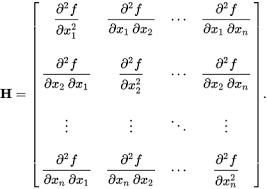
\includegraphics[scale=0.6]{fig11_14.png} 
\caption{Hessian Matrix}
\label{fig:11-13}
\end{figure}

이 과정에서 주의할 부분은 $\psi(\alpha_{i})$인데, $i$와 $j$가 서로 다를 경우 $\alpha_{j}$에 의한 미분 과정에선 상수 취급을 받지만 $i$가 $j$와 동일한 경우 하나의 변수로 미분에 영향을 주게 된다. 이에 대해 명확하게 표현하기 위해 indicator function인 $1(i=j)$를 식에 포함시켜 주었다. 

\begin{align}
\frac{d}{d\alpha_{i}d\alpha_{j}}L(\gamma,\phi|\alpha,\beta)\nonumber & = &
\frac{d}{d\alpha_{j}}[\sum^{M}_{d=1}(-\psi(\sum^{N}_{i=1}\gamma_{d,i})+\psi(\gamma_{d,i}))+M\psi(\sum^{K}_{i=1}\alpha_{i})-M\psi(\alpha_{i})]\nonumber\\
& = & M\psi^{'}(\sum^{K}_{i=1}\alpha_{i})-\psi^{'}(\alpha_{i})M1(i=j)
\end{align}

%-----------------------------------------------------------------
\subsection{Detour : Newton-Rahpson Method}
%-----------------------------------------------------------------
\begin{eqnarray}
f^{'}(x_{0}) & = & lim_{h \rightarrow 0}\frac{f(x_{0}+h)-f(x_{0})}{h}\nonumber \\
Assume \;\; r & = & (x_{0}+h)\nonumber \\
f(r) & = & f(x_{0}+h) = f(x_{0})-hf^{'}(x_{0}) \approx 0,\; if\; h \; is \; very \;small\nonumber \\
h &\approx& -\frac{f(x_{0})}{f^{'}(x_{0})} \rightarrow r = x_{0}-\frac{f(x_{0})}{f^{'}(x_{0})}\nonumber \\
x_{n+1} &=& x_{n}-\frac{f(x_{0})}{f^{'}(x_{0})}
\end{eqnarray}

Newton Rahpson method는 위와 같은 형태로 $x_{n}$에 대한 iteration을 진행해가며 특정 함수의 해를 찾아나가는 방식이다. 우리는 이 기법을 다음의 목적으로 이용하고자 한다.

\begin{figure}[ht] \centering 
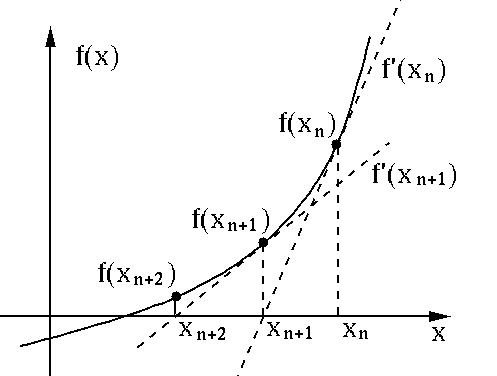
\includegraphics[scale=0.4]{fig11_15.png} 
\caption{Graphical description of Newton Rahpson Method}
\label{fig:11-14}
\end{figure}

x의 범위 속 임의의 r에 대하여 $f(r) = max_{x}f(x)$를 만족하는 f(r)은 결국 $f^{'}(r) = 0$을 만족시키는 r을 찾는 것과 같다. 즉, 우리의 Optimization 과정에서 Newton raphson method가 쓰일 수 있는 것이다. 위의 식에서 $f(x_{0})$ 대신 $f^{'}(x_{0})$을 집어넣어줌으로써 우리는 Newton raphson method를 root finding이 아닌 optimization에 이용할 수 있으며 $f^{''}(x_{0})$의 경우 hessian matrix의 형태로 볼 수 있으므로 다음과 같이 식을 나타낼 수 있다.

\begin{eqnarray}
x_{n+1} &=& x_{n}-\frac{f^{'}(x_{0})}{f^{''}(x_{0})} = x_{n}-H^{-1}(x_{n})f^{'}(x_{n})
\end{eqnarray}

\begin{eqnarray}
\frac{d}{d\alpha_{i}}L(\gamma,\phi|\alpha,\beta)\nonumber & = &\sum^{M}_{d=1}[-\Psi(\sum^{K}_{i=1}\gamma_{d,i})+\Psi(\gamma_{d,i}+\Psi(\sum^{K}_{i=1}\alpha_{i})-\Psi(\alpha_{i})]\nonumber \\ 
\frac{d}{d\alpha_{i}d\alpha_{j}}L(\gamma,\phi|\alpha,\beta)\nonumber & = &
M\Psi^{'}(\sum^{K}_{i=1}\alpha_{i})-\Psi^{'}(\alpha_{i})M1(i=j)
\end{eqnarray}

%-----------------------------------------------------------------
\subsection{Parameter optimization of Evidence Lower bound}
%-----------------------------------------------------------------
위의 과정들을 통해 ELBO의 Variational parameter와 model parameter에 대한 학습을 각각 진행해보았다. $\phi$ $\gamma$ $\beta$의 경우 정확한 값 혹은 비례관계의 형태로 closed form solution이 나왔으며 $\alpha$의 경우 closed form solution의 형태로 식이 나오지 않아 newton raphson method를 활용한 approximated optimization을 통해 parameter를 학습시킬 수 있었다. 그 결과는 아래와 같다.\\

1. Variational parameter learning
\begin{eqnarray}
\phi_{d,n,i} & \propto & \beta_{i,w_{d,n}}exp(\Psi(\gamma_{d,i}))\nonumber \\
\gamma_{d,i} & = & \alpha_{i}+ \sum^{N_{d}}_{n=1}\phi_{d,n,i}\nonumber
\end{eqnarray}

2. Model parameter learning

\begin{eqnarray}
\beta_{i,v} &\propto& \sum^{M}_{d=1}\sum^{N_{d}}_{n=1}\phi_{d,n,i}1(v=w_{d,n})\nonumber\\
\alpha_{n+1} &=&
\alpha_{n}-H^{-1}(\alpha_{n})f^{'}(\alpha_{n})\nonumber
\end{eqnarray}
\begin{eqnarray}
f^{'}_{i} & = & \frac{d}{d\alpha_{i}}L(\gamma,\phi|\alpha,\beta) = \sum^{M}_{d=1}[-\Psi(\sum^{K}_{i=1}\gamma_{d,i})+\Psi(\gamma_{d,i}+\Psi(\sum^{K}_{i=1}\alpha_{i})-\Psi(\alpha_{i})]\nonumber\\
 H_{i,j}  & = & \frac{d}{d\alpha_{i}d\alpha_{j}}L(\gamma,\phi|\alpha,\beta) = M\Psi^{'}(\sum^{K}_{i=1}\alpha_{i})-\Psi^{'}(\alpha_{i})M1(i=j)
\end{eqnarray}

위의 식에서 볼 수 있듯이 모든 parameter가 그 값을 구하려면 다른 parameter의 정보를 알아야만 한다. 이러한 정보의 필요성에 대해 network를 그려주면 다음과 같다.

\begin{figure}[ht] \centering 
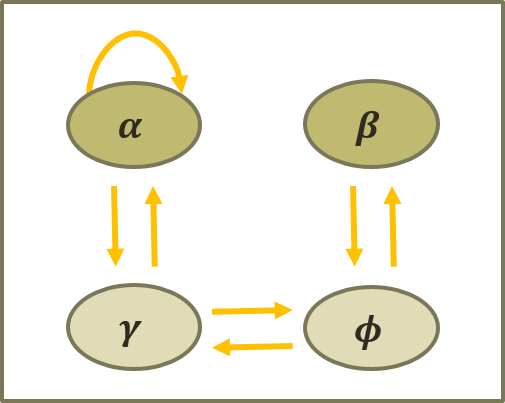
\includegraphics[scale=0.8]{fig11_13.png} 
\caption{information necessity network of parameters}
\label{fig:11-15}
\end{figure}

결국 ELBO에 대한 maximization을 위해서 우리는 parameter의 영향관계를 고려하여 각 parameter를 점진적으로 학습시키는 coordinated ascent 방식을 사용하여 각 parameter들을 학습시켜나가야함을 알 수 있다.


%-----------------------------------------------------------------
\subsection{Evaluation of LDA}
%-----------------------------------------------------------------
앞의 장을 통해 LDA model에 관한 derivation과 Variational inference의 적용을 시도해보았다. 이번 장에서는 LDA의 성능을 평가하는 방식에 대해 알아보겠다. 

대표적으로 word-topic 관계에 대한 parameter $\beta_{i,v}$는 topic i에서 word v가 가지는 설명력, 즉 확률을 나타낸다. 가령 $\beta_{t1,w1}$이 높은 값을 가진다는 것은 단어 w1이 주제 t1에 큰 영향을 주는 단어라고 볼 수 있는 것이다. 이렇듯 실제 $\beta_{i,v}$의 분포를 사람이 직접 확인하면서 평가하는 방식이 가능하며 이는 정성적인 평가방식이라 할 수 있다. 

이와 반대로 LDA의 정량적인 평가방식은 $lnP(w_{d}|\alpha,\beta)$를 이용하는 것이다. 이 확률은 곧 주어진 $\alpha$, $\beta$에 대한 Document data의 확률이라고 볼 수 있다. 위의 확률이 학습을 진행함에 따라 얼마나 높아지는 지에 대한 추이와 정도를 파악하여 LDA의 성능을 측정할 수 있다.

\end{document}
